%include polycode.fmt 
%format |-> = "\mapsto"
%format veca = "\vec a"
%format vecb = "\vec b"
%format delay1 ="\sigma_1"
%format delayx ="\sigma_x"
%format delay = "\sigma"
%format Delayx = "\Delta_x"
%format Delay1 = "\Delta_1"
%format mylang = "\lambda^{\rightarrow}_{\Delta}"
%format psin = "\psi. n."
%format < = "\langle"
%format > = "\rangle"
%format *> = ">"
%format <--> = "\leftrightarrow"
%format <- = "\leftarrow"
%format -!> = "\overset{!}{\rightarrow}"
%format \\ = "\lambda"
%format <==> = "\leftrightarrow"
%format <||> = "\langle || \rangle"
%format par = "\langle || \rangle"

\chapter{Formalization}
\chapter{Semantics of Time}
In this chapter we will introduce a type-system based on constraint based typing as introduced in the previous chapter.
While we will re-introduce basic notation used in defining our typing rules, we will not explain the workings of constraint based typing, the $\lambda$-calculus and type-systems in general in this chapter.
If these concepts are unfamiliar, the previous chapter may be used as an introduction. 

Our type-system will use constraints to limit the temporal behaviour of hardware descriptions.
Whether or not this can be rightfully called a type-system is open for discussion.
In this thesis however we consider temporal constraints as a type-system, as the purpose of other type-systems and our temporal constraints are similar.
Moreover, when timing behaviour is subject to constraints we can reason about circuit descriptions together with their temporal limitations.
Like types, temporal constraints express a limitation on expressions.
In that light we consider our system a type-system.
However, even though our type-system is similar to constraint-based typing we will not discuss a combination of the two until after introducing our system. 
As such, certain identifiers, as introduced in the previous chapter, may be reused whenever they describe similar things. 

To introduce our type-system we will first give a general introduction as to what is currently possible using a system like the simply typed $\lambda$-calculus.
After doing so we will first give an informal overview of our type-system and how we constraint time of components in hardware designs.
Following this informal understanding of our model of time we will extend the grammar of the constraint based $\lambda$-calculus and provide typing rules which express the relation between types and terms.
Afterwards we will define what it means for a term to be well-typed, together with an informal method to show that timing constraints hold.

\section{Introduction}
Even though the untyped $\lambda$-calculus can be used as a foundation to elegantly express computations, as shown by programming languages such as Haskell\cite{jones2003haskell} and Lisp\cite{mccarthy1965lisp}, the untyped $\lambda$-calculus by itself is not suited as a method to reason about the physical constraints which these computations may be subject to.
When describing hardware we do not want to limit ourselves to expressing only computations, but we also want to express when, where and how these computations are executed.
To allow accurate reasoning about the behavior of a circuit description we must be able to express all of these constraints accurately and in an intuitive manner.
Without being able to do so the complexity of the system soon catches up with our ability to express interactions and all added advantages of expressing temporal behavior are surely lost.

The simply typed $\lambda$-calculus is able to more specifically limit computations.
However, we are still not able to specify when these computations occur, nor where these computations occur.
For hardware description the simply typed $\lambda$-calculus is, expressive enough to specify the following:
\begin{itemize}
 \item Data representation in terms of bits, provided base types are created for every type of data.
 \item Hierarchically organise computations through abstraction and application.
\end{itemize}

Additionally, \citeauthor{clashchris} and \citeauthor{kooijman2009haskell} have explored\cite{clashchris,kooijman2009haskell} ways to translate a dialect of the $\lambda$-calculus to \gls{vhdl}.
Their approach exposes parallelism from the Haskell Core language and is essential in generating hardware from a hardware description which uses the $\lambda$-calculus.
As such we can conclude that the simply typed $\lambda$-calculus can express parallelism implicitly.
Their approach also shows $\beta$-reduction is preserved during translation to \gls{vhdl}, which represents the computational aspect of the $\lambda$-calculus.

What is not possible is to specify when and where these computations take place.
We can easily abstract from the latter, as synthesis tools are sufficiently advanced to make manual placement, at least in the general case, unnecessary, but we cannot specify directly when these computations take place.
Furthermore, if we are able to specify when computations take place then we would also like to have a certain degree of verification when creating compositions of computations. 
For this reason we will introduce a modified version of constraint-based type-checking.
We will allow a hardware designer to define components independently and then, through composition and primitive, temporal operations, allow the type-system to verify whether the composition still behaves correctly.
Before doing so however we need a sense of time, which we will present in the next section.


%%%%
% Time Representation
%%%%
\section{Time Representation}
As mentioned in the previous chapter, the synchronous approach is used most commonly for hardware description.
Since this is the case, and since \gls{clash} is already considered a synchronous language, we limit ourselves to the synchronous approach here.
To introduce the concept of timing constraints we first limit ourselves to combinational logic and general observations while ignoring the details of the synchronous approach first, before introducing memory elements and differences in sample speeds.

\begin{figure}[h]
\begin{minipage}{0.45\textwidth}
\centering
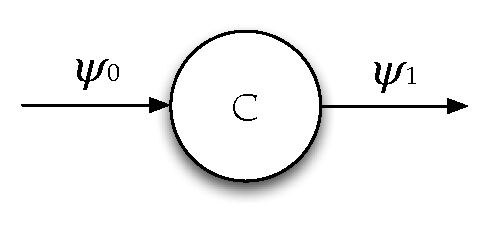
\includegraphics[width=\textwidth]{images/comp}
\end{minipage}
\begin{minipage}{0.45\textwidth}
\centering
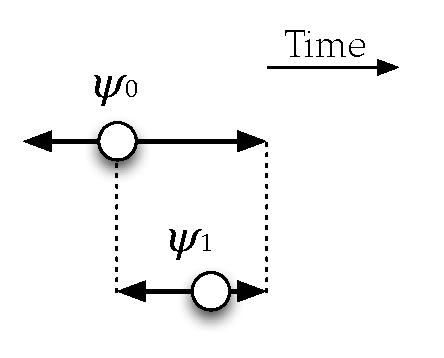
\includegraphics[width=0.8\textwidth]{images/constraintsingle}
\end{minipage}
\caption{A single component together with its time variables} \label{fig:singlecomp}
\end{figure}

First, in order to be able to reason about time we introduce the concept of a \textit{time variable}. 
Time variables represent moments in time which do not change within the scope of expressions where they are used in; within a single scope time variables are constants.
This is similar to mathematical variables, such as in $f(x) = x^2$, where $x$ is considered a constant \textit{within} the scope of $f$.
We will use $\psi$ to range over time variables.
When we define a certain component $C$, as shown in figure \ref{fig:singlecomp}, every input and output of the component is associated with a distinct time variable.
Without looking at the component definition we can deduce, in order to maintain causality, that $\psi_0$ must precede $\psi_1$ in time, or must occur at exactly the same time as $\psi_0$.

When we limit ourselves to combinational logic the time difference between $\psi_0$ and $\psi_1$ represents the length of the critical path in $C$.
We can express the relation between $\psi_0$ and $\psi_1$ through a timing diagram, shown in figure \ref{fig:singlecomp}
The time variable $\psi_0$ depends on the input provided to this component.
When we soley consider this component we do not know when the input is actually available.
This is represented as the black arrow in the timing diagram, which represents all moments in time which $\psi_0$ can represent.
When solely considering $C$, $\psi_0$ is unrestricted and as a result we can pick \textit{any} point in time and replace $\psi_0$ with it.
This influences the possible position in time of $\psi_1$ however, as $\psi_1$ depends on $\psi_0$. 
To express this we pick a specific instance of $\psi_0$, indicated by the small circle on the black arrow labelled $\psi_0$.
The time variable $\psi_1$ depends on $\psi_0$, which is expressed as the dotted line between the start of all possible positions of $\psi_1$.
When we know nothing of $C$ the critical path is variable, as it depends on the definition of $C$. 
We express this as the difference in time between $\psi_0$ and $\psi_1$ by also picking a specific instance for $\psi_1$.
Since we are limiting ourselves to combinational logic, $\psi_0$ must occur within the same clock-cycle as $\psi_1$, which is represented by the dotted line between the endpoints of both arrows.
Timing diagrams such as these can be used to reason about temporal effects under changing conditions.
We can imagine moving the instance of $\psi_0$ horizontally and imagine the effects it has on $\psi_1$.

While timing diagrams are useful, they are not suited to concisely represent temporal constraints.
To do so we can create relations between time variables symbolically. 
For instance, the relation as shown in figure \ref{fig:singlecomp} can be expressed as $\psi_0 \le \psi_1$.

%
% Time variables and Relations
%
\begin{definitiontitled}[text only,float]{Time variables and Relations}{def:timevar}
A \textbf{time variable}, denoted $\psi_0 \ldots, \psi_n$, represents a moment in time.
Two time variables may be related to each other in the sense that one must always precede the other, or occur at exactly the same time.
\end{definitiontitled}


We can use relations such as $\psi_0 \le \psi_1$ to define a mapping to hardware, as shown by figure \ref{fig:constraintsinglemap}, where a single component can be used to handle input streams, without directly using streams in its definition.
When we take the natural numbers, including 0, as representing time instances, then we can replace $\psi_0$ with any $n \in \mathbb{N}_0$, as shown in the timing diagram.
Moreover, since we know nothing of $\psi_1$ in relation to $\psi_0$ other than the latter must precede the former, we can replace $\psi_1$ with any $n \in \mathbb{N}_0$ provided $\psi_0 \le \psi_1$. 
Using these relations we can map a component over time, as shown by figure \ref{fig:constraintsinglemap}.
The time between $\psi_0=n$ and $\psi_0=n+1$ determines the length of a single period.
We have indicated this in the diagram by transparent arrows between $\psi_1 = 0$ and $\psi_1 = 1$.
The length of time between these indicates the length of a single clock-cycle in a synchronous circuit.

\begin{figure}[h]
\centering
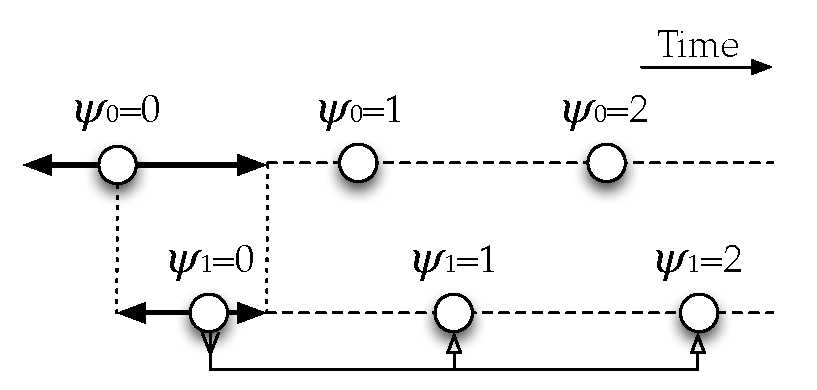
\includegraphics[width=0.6\textwidth]{images/constraintsinglemap}
\caption{A mapping of a component's time behaviour to a stream} 
\label{fig:constraintsinglemap}
\end{figure}

\subsection{Timing Constraints}
Relations between two time variables, such as $\psi_0 \le \psi_1$, are called timing constraints. 
These can be deduced automatically when two components are composed.
Shown in figure \ref{fig:dualcomp} are two components, each with their own time variables.
When we compose the two we can deduce that $\psi_0 \le \psi_1$, $\psi_1 \le \psi_2$ and $\psi_2 \le \psi_3$.
However, we have mentioned before that we limit ourselves to combinational logic as well as the synchronous approach.
Based on those two assumptions we could be more strict in the sense that $\psi_0 = \psi_1 = \psi_2 = \psi_3$.
When we introduce sequential logic we can no longer assume every component consists of combinational logic however, and as such we do not make any such assumption here either.
When we want to indicate however that a component \textit{does} in fact consist solely combinational logic we will use the same time variable for all inputs and all outputs, as shown in figure \ref{fig:constraints1circuit}.

\begin{figure}[h]
\centering
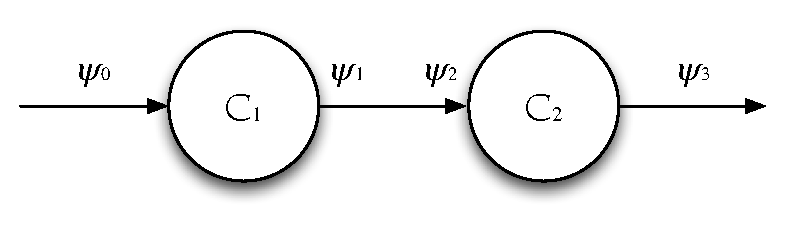
\includegraphics[width=0.65\textwidth]{images/compcomp}
\caption{Two components composed together with their time variables} \label{fig:dualcomp}
\end{figure}

Timing constraints are created using the $\le$ operator, which does not define \textit{exactly} when moments occur in relation to each other, but only introduces an ordering of computations in time.
To clarify this concept we will introduce a small sub-component of a circuit in figure \ref{fig:constraints1circuit}.
Each of these components $C_0 \ldots C_2$ represent combinational logic, and as such each component has its own associated timing variables $\psi_0 \ldots \psi_2$.
For demonstrative purposes we will ignore the inputs and outputs of this circuit.

\begin{figure}[h]
\centering
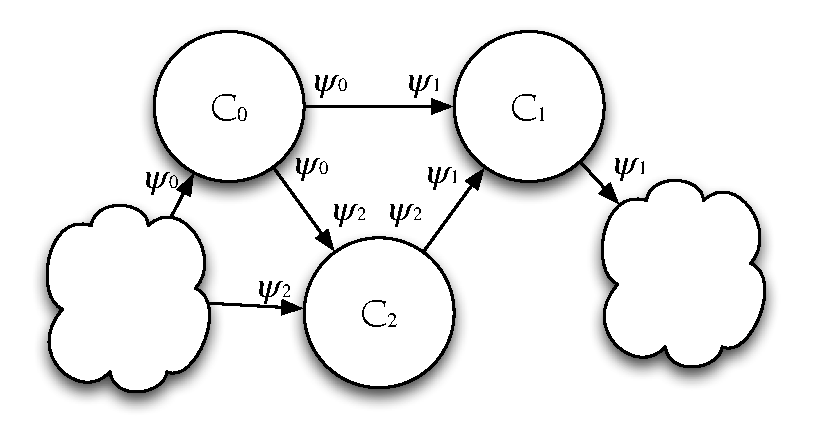
\includegraphics[width=0.65\textwidth]{images/constraints1circuit}
\caption{A composition and its constraints}
\label{fig:constraints1circuit}
\end{figure}

To model the difference between distinct clockcycles, whenever a moment in time labelled $\psi$ occurs, $\psi + a$ with $a \neq 0$ can not occur.
The constant $a$ represents the phase difference of $\psi$ when compared to $\psi+a$.
As a result, when using combinational logic which is supplied with data at $\psi$, we can never observe data for any moment $a \neq 0$ in $\psi + a$.
This effect is made visible in figure \ref{fig:constraints1} by adding $\psi_0 + 1$ as an upper bound for possible positions of $\psi_0$ relative to other time variables.
Similarly, $\psi_0 - 1$ is a lower bound.

\begin{figure}[h]
\centering
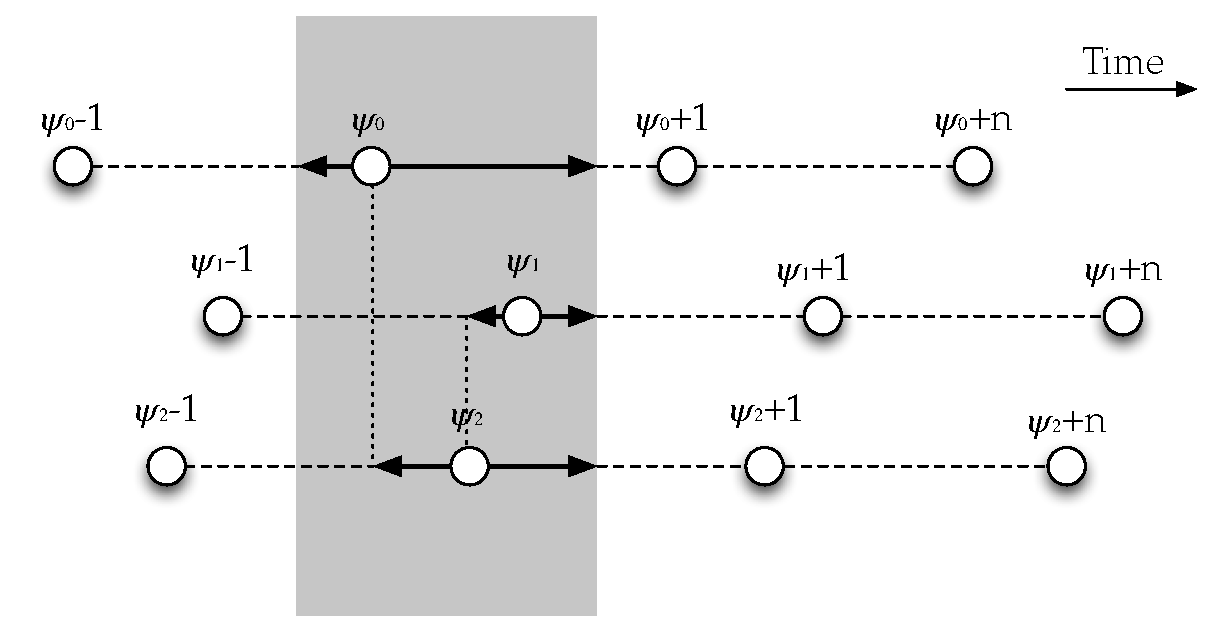
\includegraphics[width=0.65\textwidth]{images/constraints1}
\caption{Time constraints of the composition from figure \ref{fig:constraints1circuit}}
\label{fig:constraints1}
\end{figure}

In this timing diagram we started by defining the moment $\psi_0$.
Like earlier, this time variable is unrestricted.
Since $C_2$ depends on $C_0$ this means that $\psi_2$ may never precede $\psi_0$, as indicated by the dotted line between $\psi_0$ and the start of all possible positions of $\psi_2$.
As all components consists only of combinational logic this means that it restricts both $\psi_0$, $\psi_1$ and $\psi_2$ to be available within the same clockcycle.
This is illustrated by the gray rectangle in figure \ref{fig:constraints1}.
Alternatively we can illustrate this via the constraint $\psi_2 \le \psi_0 + 1$, as well as the constraints $\psi_0 \le \psi_2$ and $\psi_1 \le \psi_0 + 1$. 
The constraint $\psi_0 \le \psi_0 + 1$ always holds, since $\psi_0 < \psi_0 + 1$ is axiomatically true.

The restriction of time variables by composition shows how behaviour in time depends on the context in which a component is used.
For instance, if we were to use this composition in another composition where $\psi_2 \le \psi_0$, then clearly $\psi_2 = \psi_0$. 
This does not matter greatly yet, since we limited ourselves to combinational logic.
If the most restricting timing constraint is equality, then combinational logic can always be expressed.
However, if we were to express sequential logic, then we can use constraints such as these to check if compositions behave sanely.
To do so however, we will need to introduce memory elements and the timing model of sequential logic.

%The timing constraints we introduced are very familiar to the typing constraints from the previous chapter.
%There, we introduced a set of typing constraints of the form $\tau = \sigma$, where $\tau$ and $\sigma$ represent types.
%Similarly we also introduce a set of timing constraints in definition \ref{def:constraintpsi1}.
%We use the already introduced time expression $\tau$ in our constraints, as each time expression consists of at least one time variable $\psi$ and can therefor express the constraints.
%
%\begin{definitiontitled}[text only,float]{Set of constraints $\mathcal{C}$}{def:constraintpsi1}
%Let $\tau$ and $\sigma$ be time expressions with associated variables $\psi_\tau$ and $\psi_\sigma$ and offsets $a$, $b$, then the $i^{th}$ \textbf{time-constraint} $\mathcal{C}_i$ is defined as an element of the set $\mathcal{C}$ as follows:
%\[
%\mathcal{C}   = \{\mathcal{C}_i | i \in 1..n\} \quad \\
%\mathcal{C}_i = \tau \le \sigma 
%\]
%, where $\le$ is the non-strict ordering relation between $\tau = \psi_\tau + a$ and $\sigma = \psi_\sigma + b$.
%\end{definitiontitled}

%To avoid confusion over the previous sections and the next section we do allow relations as $\psi_0 \le \psi_1$.
%Whenever time variables themselves are used in inequality relations they can be converted to a time constraint by defining $\tau = \psi_0$ and $\sigma = \psi_1$.
%

\subsection{Lifetime}
Since we have defined upper and lower bounds to time variables, like in figure \ref{fig:constraints1}, we have also defined an interval of time where a value exists.
The interval of time during which a value is valid is called the \textit{lifetime} of a value.
We can determine the difference in lifetime between two values if the \textit{rate of change} is known.
For now we will only consider a constant rate of change, which means we can relate this rate of change to a single clock.
In synchronous hardware description a clock is used to indicate the passage of time.
Using this clock we can define the minimum lifetime of a value, as it is at least equal to one period of the clock. 
The rate of change of the clock is twice as fast as the values which are synchronised to it, as a clock alternates between two distinct states.

When we relate a changing value to a clock then we can also define when a value changes.
Figure \ref{fig:lifetime} shows how the length of the clock, labelled \textit{clk}, can change depending on when an abstract moment in time, labelled $\psi_0$, occurs.
Not only does it depend on $\psi_0$, but also on another moment which we label $\psi_0 + 1$.
This time variable is phase shifted in comparison to $\psi_0$. 
The length of time between $\psi_0$ and $\psi_0+1$ is, for the purposes of discussing lifetime at least, completely variable. 
We can choose $\psi_0$ and as a result the rate of change of the value associated with $\psi_0$ is increased.

\begin{figure}[h]
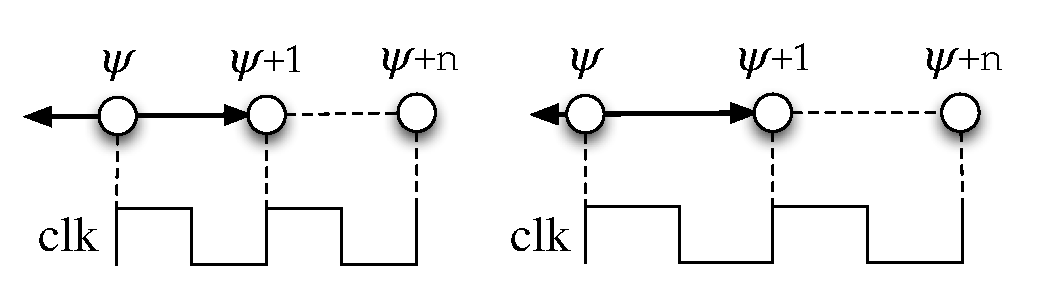
\includegraphics[width=0.8\textwidth]{images/lifetime}
\centering
\caption{Length of a clockcycle, which depends on time variables.} \label{fig:lifetime}
\end{figure}

For realistic circuits the limitation of a fixed rate of change might seem overly restrictive, as hardware description languages generally have the ability to up or downsample a signal, but for now we will focus on immutable rates of change.
When we know the minimum lifetime of values we can also, in principle at least, determine when components are used, and how compositions of components \textit{should} be used in order to maintain $\beta$-reduction.
This may seem like a tall order, but before we can show meaningful examples we first introduce memory elements.

\subsection{Memory Elements}
We can also use the lifetime of values to reason about memory elements.
Memory elements can be seen as bridges between time instances.
Figure \ref{fig:dff} shows a D flip-flop, which is trigged by a periodic clock or a set/reset toggle, together with a timing diagram.
The data input, labelled D, is available at $\psi$.
Since a D flip-flop is triggered by a periodic clock, named clk, whenever data is supplied to the input at $\psi$, the same data will be available at the output Q precisely at $\psi+1$, which is the next clock cycle of the associated clock $clk$.
We can express this memory element through the addition operation, as shown by figure \ref{fig:dff}.
When we add an offset to a time variable we specify how many memory elements should be inserted.
When we pick $\psi = 0$ first, then in the example diagram $D$ will have the value $42$. 
The value of $Q$ will be the same as $D$, only one moment in time later, namely when $\psi=1$.

\begin{figure}[h]
\centering
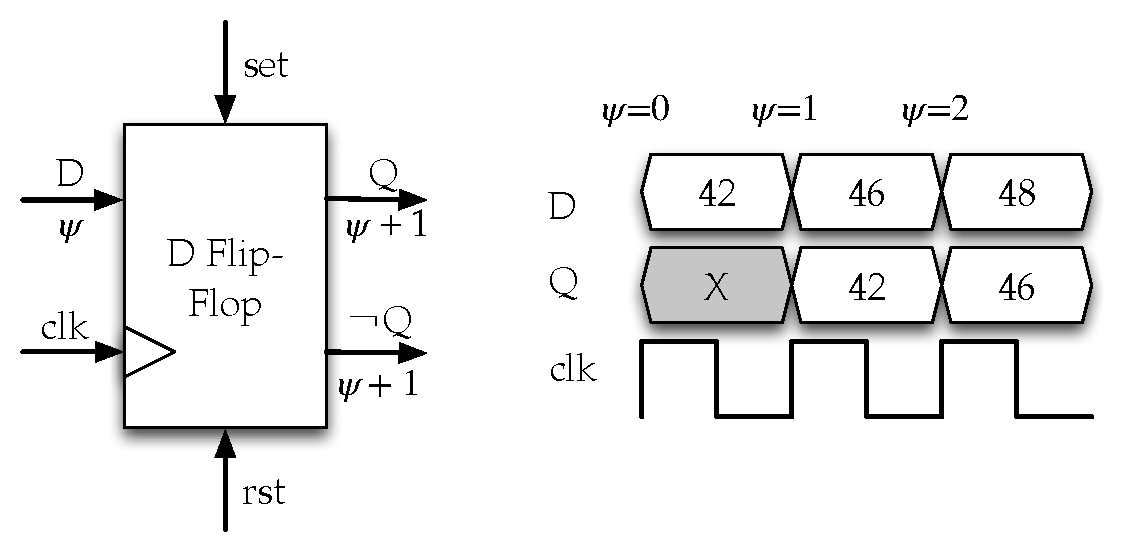
\includegraphics[width=0.7\textwidth]{images/dff}
\caption{A D Flip-Flop and its behaviour in time} \label{fig:dff}
\end{figure}

As shown by the D flip-flop, we use the same time variable for both the input as the output.
This is the only way how memory elements can be introduced through time variables.
Time variables refer to a fixed rate of change, which means each time variable has an associated lifetime.
Since we reference the same time variable for both the input and output of the memory element we also bind the lifetime of the input value to the lifetime of the output value. 
This makes sense in hardware since changes in the memory element are toggled by a single clock.
This single clock also relates the input to the output in the sense that the output is always produced one cycle after the input, and as such exists one time unit later.

\subsubsection{Time Expressions}
So far we have only dealt with time variables $\psi$.
Similar to the relation between type variables and types, we introduce \textit{time expressions} in definition \ref{def:timeexpr1}.
Unlike the relation between type variables and types, time expressions \textit{always} contain time variables. 
An operation such as $+$ could be seen as a time expression constructor, similar to how $\rightarrow$ is a type constructor.

\begin{definitiontitled}[text only,float]{Time Expression (1)}{def:timeexpr1}
This is indicated by the arrow, which indicates the interval from which we may choose $\psi_0$.
We allow operations, such as addition on time variables leading to \textbf{time expressions}.
Like types, we use $\tau, \sigma, \rho$ to range over time expressions.
Addition of a constant offset to a time variable as in $\psi + a$, is defined as expressing the time expression $\tau= \psi + a$, where $\psi + a$ can always be replaced by $\tau$ and vice versa.
\end{definitiontitled}

Time expressions allow us to move memory elements around without affecting the behaviour of the circuit.
Since we have not defined the initial content of memory elements we can still move memory elements indescriminately; the circuit is subject to \textit{retiming}.
As an example we define an adder component as in figure \ref{fig:timedadder}, with the constraints $\psi_0 \le \psi_2$ and $\psi_1 \le \psi_2$.

\begin{figure}[ht]
\begin{minipage}[b]{0.375\linewidth}
\centering
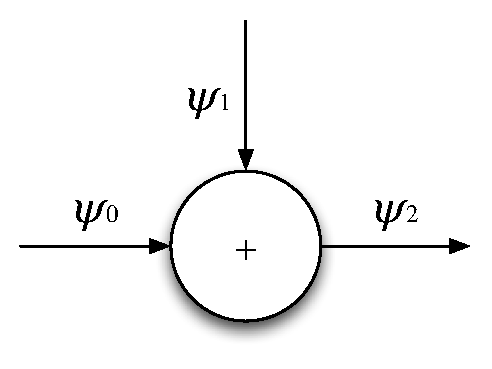
\includegraphics[width=0.9\textwidth]{images/adder}
\caption{A timed adder with the constraints $(\psi_0,\psi_1) \le \psi_2$}
\label{fig:timedadder}
\end{minipage}
\hspace{0.5cm}
\begin{minipage}[b]{0.625\linewidth}
\centering
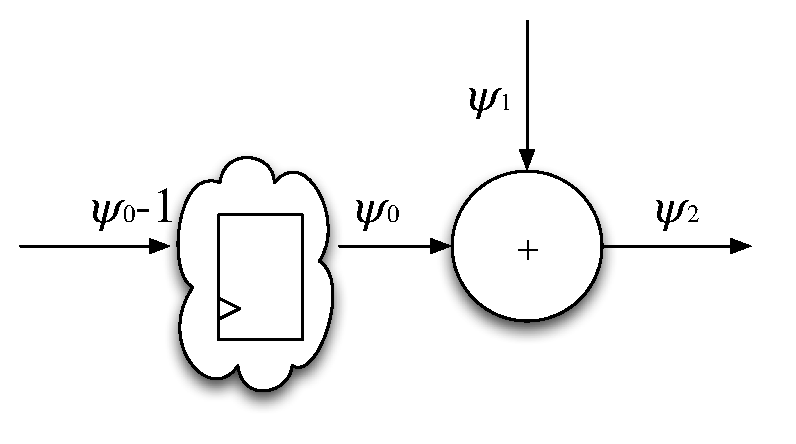
\includegraphics[width=0.9\textwidth]{images/addermemory}
\caption{A timed adder with the addition constraint $\psi_0 \le \psi_1 + 1$}
\label{fig:timedaddermemory}
\end{minipage}
\end{figure}

As the rate of change in the environment is fixed, we know that whenever $\psi_0$ changes, $\psi_1$ must also change.
When we introduce the additional constraint $\psi_0 \le \psi_1 + 1$, then in order for the addition operation to work properly the input labelled $\psi_0$ must be delayed \textit{somewhere} before being supplied to the addition operation.
How the constraint $\psi_0 \le \psi_1 + 1$ is created in the environment is of no concern, as long as the constraint is taken care of at some point.

%%%%
% Functions as values
%%%%
\subsection{Functions as Components}
Since we are using the functional paradigm functions are values as well.
We are using functions as an equivalent to hardware components.
Unfortunately, hardware components cannot be considered values, since we cannot transfer them over wires.
In order to reason about functions as components, without losing the ability to have first-class functions, we we must explore how components relate to time as if components were values themselves.
To do so we need to clarify part of the type-system of $\lambda^\rightarrow$ however, as it clarifies in what way the type-system provides the ability of first-class functions.

We take the addition function as an example.
Restricting ourselves to integer inputs the type of $f$ would be $Int \rightarrow (Int \rightarrow Int)$.
This means that $f$, when applied to the first argument, will produce a new function $f'$, which has type $Int \rightarrow Int$.
As functions are values we can also annotate these with time variables.
Let $C$ be the component representation of $f$, then $C$ ``produces'' a second component $C'$ which is able to be applied to another argument as shown by figure \ref{fig:2arycomp}.
The input of $C$ arrives at $\psi_0$, then the component $C'$ is instantly produced at $\psi_1$.
The component $C'$ can then use an input $\psi_1$, which is \textit{unrelated} to $\psi_0$.
Finally, $C'$ will produce a value, which will be available at $\psi_2$ under consideration that $\psi_0 \le \psi_2$ and $\psi_1 \le \psi_0$.
As a result, function values do not have to behave causally.
When the second argument in our example, labelled $\psi_1$, arrives earlier than $\psi_0$, then the function is moved backwards in time.
This is of no concern, as functions can not be considered \textit{real} values anyway; we can never move a function over a wire.

\begin{figure}[h]
\centering
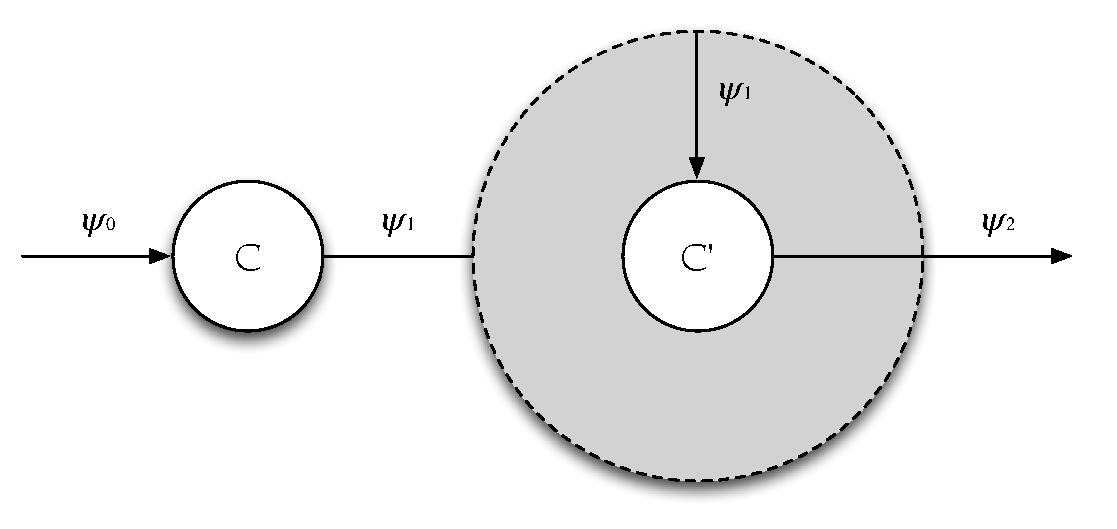
\includegraphics[width=0.8\textwidth]{images/2arycomp}
\caption{A component which produces another component.} \label{fig:2arycomp}
\end{figure}

The relation between functions and hardware components is somewhat difficult, as the components the functions represent necessarily exist in continuous time.
However, we are not interested in the results of functions at \textit{every} continuous time instance, we are merely interested in results of functions at \textit{specific} time instances.
As such we are not interested in function definitions at every time instance either, as long as they are well behaved at the time instances at which we expect it to be well-behaved.
With this in mind we can consider functions as values, even in the domain of hardware, provided functions themselves are not subject to the same restrictions as real values.
The components which represent functions do exist, yet the functionality they represent is only known to be correct at specific instances. 
At other moments in time the functionality may also be correct, but from a language point of view we make no assumptions on whether or not this should be the case.

%%%%
% Context and Composition
%%%%
\subsection{Context and Composition}
As mentioned earlier, whenever we use application to compose values we make an assumption on the validity of the values we are composing, independent of the rest of the circuit definition.
This does not mean we cannot define functions where two abstract events are not related, as shown by figure \ref{fig:indepcomp}.
There we show two components $C_1$ and $C_2$, each with independent time variables.
Referring only to the composition of these two components we cannot see how $\psi_0$ and $\psi_2$ relate.
However, as we do not allow upsampling and downsampling yet, we are able to determine the relative offsets between $\psi_0$ and $\psi_2$ using the context in which the component is used.
As a result, we are able to define the behaviour of both $C_1$ and $C_2$ in relation to eachother.


\begin{figure}[h]
\centering
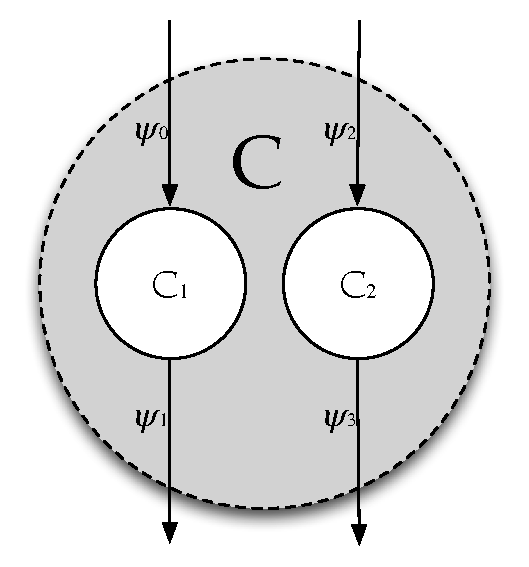
\includegraphics[width=0.5\textwidth]{images/indepcomp}
\caption{Two independent components in a single composition.} \label{fig:indepcomp}
\end{figure}

While we cannot say anything about $C_1$'s relation to $C_2$, we can certainly say that such a relation must exist somewhere in the context where the composition $C$ is used in.

%%%%
% Flexible and Strict constraints
%%%%
\subsection{Flexible and Strict Constraints}
So far we have not properly defined how constraints can be interpreted.
We can define at least two ways in which we can interpret constraints. 
Later on we will define a few other ways in which we could interpret constraints, but for now we will focus on \textit{strict} and \textit{flexible} constraints.
First we will define flexible constraints through an example, after which we will introduce a way to create strict constraints.

\subsubsection{Flexible Constraints}
Shown in figure \ref{fig:bigcomp} is a composition with components $C_0 \ldots C_3$ and associated time variables $\psi_0 \ldots \psi_4$.
From the time variables we can assume that $C_2$ is combinational, as it is only associated with a single time variable.


\begin{figure}[h]
\centering
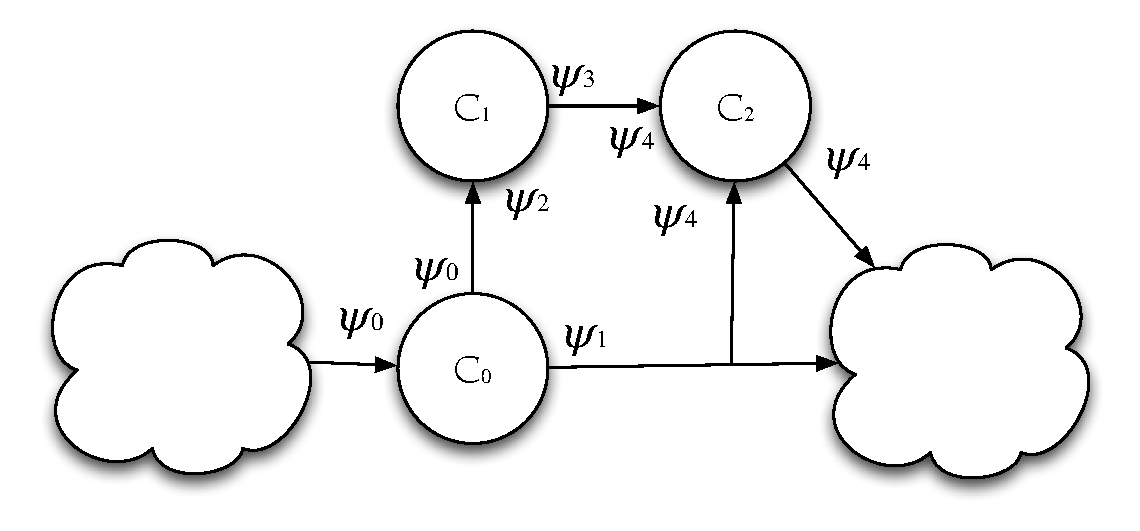
\includegraphics[width=0.6\textwidth]{images/bigcomp}
\caption{A simple composition of two unknowns and one combinational component} \label{fig:bigcomp}
\end{figure}


By itself this does not have any effect on the composition.
However, this changes when we add the constraint $\psi_0 \le \psi_1 + 1$, which indicates that somewhere between the input of $C_0$ and the output labelled $\psi_1$ a memory element needs to be added \textit{without} affecting the other output labelled $\psi_0$.
To clarify this we added a timing diagram, shown in figure \ref{fig:bigcomptiming}, which shows how the additional constraint relates time variables $\psi_0 \ldots \psi_4$ to each other.
When we do not yet know anything about $C_1$, $\psi_2$ and $\psi_3$ are limited by $\psi_0$ and $\psi_4$.
If we assume $C_1$ only contains combinational logic, then $\psi_2$ and $\psi_3$ have to occur during the lifetime of $\psi_0$, in turn solely limiting $\psi_2$ and $\psi_3$ by $\psi_0$.


\begin{figure}[h]
\centering
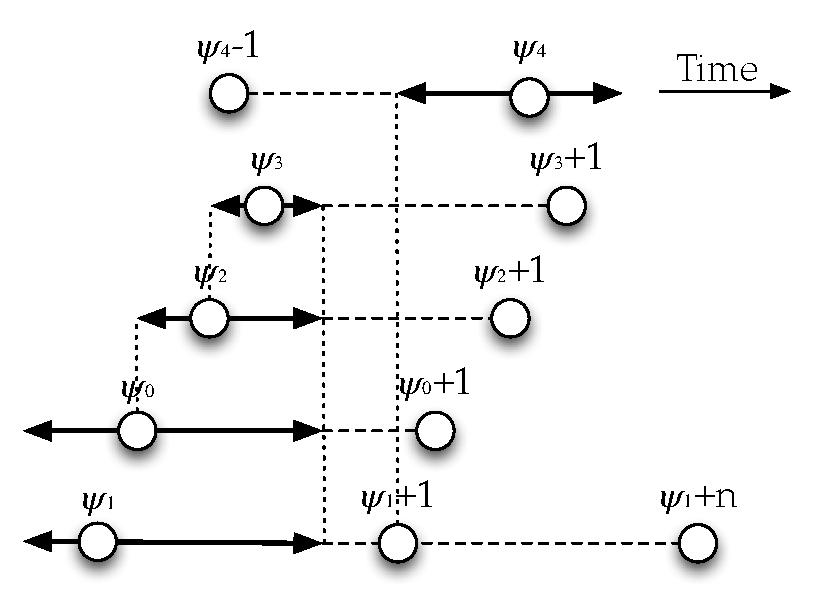
\includegraphics[width=0.65\textwidth]{images/bigcomptiming}
\caption{Timing diagram of figure \ref{fig:bigcomp}} \label{fig:bigcomptiming}
\end{figure}


We have rewritten the composition of figure \ref{fig:bigcomp} to include a memory element, as shown in figure \ref{fig:bigcomprewritten}.
To maintain the functionality described by $C_2$, which defines both inputs to be available at the same time, a memory element between $C_2$ and $C_0$ along the path of $C_1$ must be present.
To do so we may insert memory elements where we need to, as all other relations are flexible: $\psi_0 \le \psi_2 \le \psi_3$ et cetera.
However, $C_1$ may also include a memory element already, in which case we do not have to add memory elements anywhere in the composition.
What is important is that $C_2$ is defined to be completely combinational.
Whenever we compose it with other components we have the choice to implicitly add a memory element in order to maintain the behaviour within $C_2$.
Assuming this is the case, then the composition needs to be changed to maintain the functionality described in $C_2$.
This means that the environment which $C_2$ is used in is responsible to provide synchronized inputs, regardless of the computational paths leading up to the inputs of $C_2$.

\begin{figure}[h]
\centering
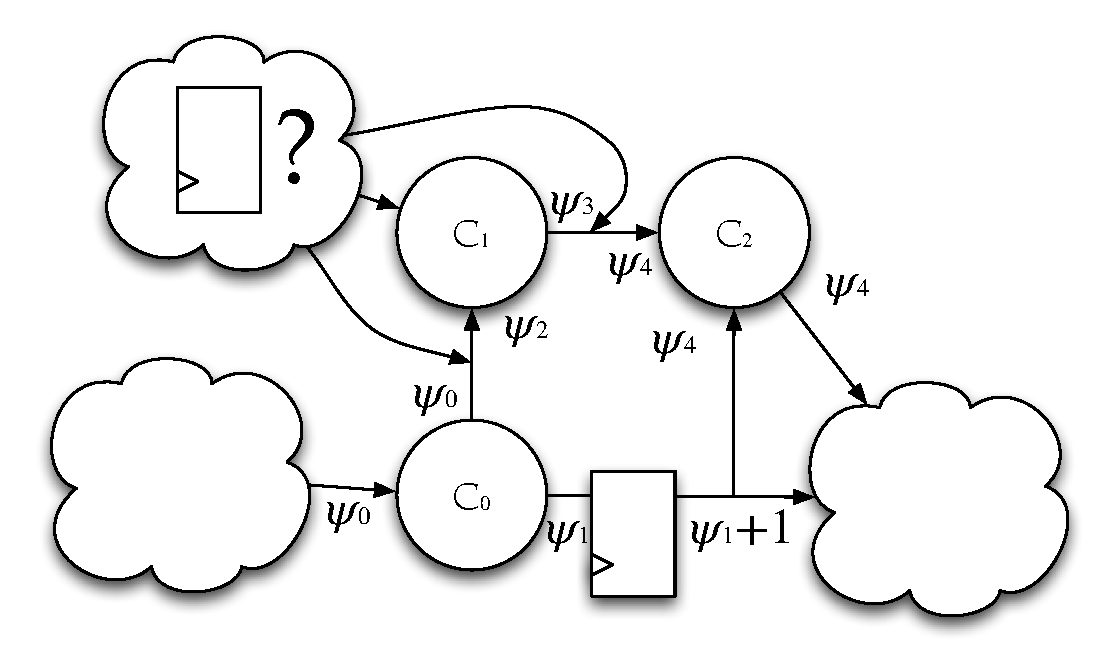
\includegraphics[width=0.75\textwidth]{images/bigcomprewritten}
\caption{Possible locations of additional logic under constraints} \label{fig:bigcomprewritten}
\end{figure}

Alternatively we could give an error message which informs the designer that a mismatch is introduced within this composition.
Either way, we control the timing behaviour of compositions.
What this example should make clear however, is that timing behaviour of individual components have an effect on compositions they are used in.
Building from individual components allows us to check the timing behaviour of the composition, assuming of course we want to maintain the timing behaviour for each component individually.




\subsubsection{Strict Constraints}
So far we have only limited expressions using the $\le$ operation.
The $\le$ operation between two time variables is not strict and allows the type system to add all the memory elements needed to make the composition work.
However, this might be too flexible for all forms of hardware description.
Sometimes a more strict verification of timing is required, especially in areas where latency is important.
To allow more strict verification of timing we first introduce the $\delta$ operation as in definition \ref{def:delta}.

\begin{definitiontitled}[text only,float]{$\delta$-function for delays}{def:delta}
The $\delta$\textbf{-function} inserts a delay with a strict constraint.
In a binding as $\textbf{let } y = \delta(x)$, the variables $y$ and $x$ are associated with timing variables $\psi_y$ and $\psi_x$. 
As the $\delta$-function is used the constraint $\psi_y = \psi_x + 1$ is added.
\end{definitiontitled}

There are multiple ways in which the $\delta$-function could influence the constraints in a design.
The first is to simply add the strict constraint as per definition \ref{def:delta} and leave the rest to be non-strict.
Another solution is to make strictness infectious. 
By this we mean that, whenever a $\delta$-function is used, everything that is composed together with this $\delta$ function must also use a strict constraint.
For now we consider this to be too restrictive, as in the current system this would mean that, once a single $\delta$-function is used, all other memory elements must also be introduced through $\delta$-functions, as the $\delta$-function is the only method to introduce a strict constraint.

%%%%
% Rate changes
%%%%
\subsection{Rate Changes}
Up until now we did not allow changes in the rate of change.
Using a rate $r$, we can relate the rate of change associated with one time variable to another time variable.
We extend the timing expression $\tau$ to include the rate in definition \ref{def:timeexp2}.

\begin{definitiontitled}[text only,float]{Time Expression (2)}{def:timeexp2}
We allow operations, such as addition and multiplication on time variables leading to \textbf{time expressions}.
Addition of a constant offset to a time variable as in $\psi + a$, is defined as creating the time expression $\tau= \psi + a$, where $\psi + a$ can always be replaced by $\tau$ and vice versa.
Additionally we allow the multiplication of a time variable with a rate $r \in \mathbb{N}_0$ within a time expression.
Time expressions are left associative, which means $3 \cdot \psi + a$ ought to be interpreted as $(3 \cdot \psi) + a$.
\end{definitiontitled}

This means that, like offsets in time variables, the rate of change is only known in terms of other time expressions.
As an example, suppose we have the circuit of figure \ref{fig:ratechange}.
In this example we take one input, which is a natural number and output three consecutive numbers at a rate which changes three times as fast as the input.
The first number is left intact, while the two numbers following it are added to four and two respectively.
Effectively the output is a sequence of values, expressed via the expression $\langle 3 \cdot \psi, 3 \cdot \psi + 1, 3 \cdot \psi + 2 \rangle$.

\begin{figure}[h]
\centering
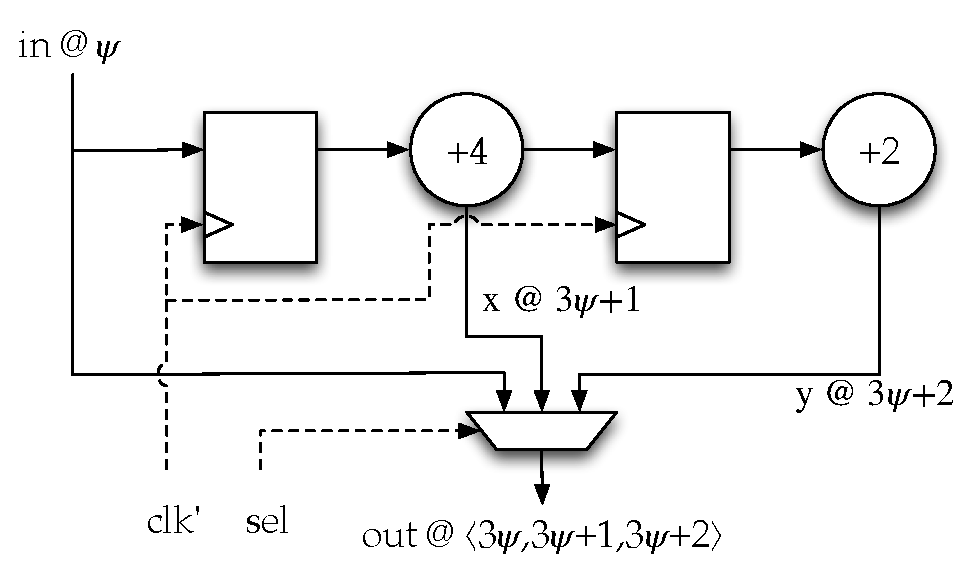
\includegraphics[width=0.6\textwidth]{images/ratechange}
\caption{An upsampling circuit}
\label{fig:ratechange}
\end{figure}

In this circuit we use a single time variable, which is multiplied with a factor three in certain expressions.
This relation is made clear in the timing diagram of \ref{fig:constraintsup}.
We can see how $3 \cdot \psi$ is constrained to $\psi$.
However, as $3\cdot \psi$ changes three times as fast this means that between $\psi$ and $\psi + 1$ the moments $3 \cdot \psi$, $3 \cdot \psi +1$ and $3 \cdot \psi+2$ also occur.
This also makes clear why time expressions are considered left associative, as the offset $+2$ in $3 \cdot \psi + 2$ refers to $3 \cdot \psi$, not $\psi$ alone.

\begin{figure}
\centering
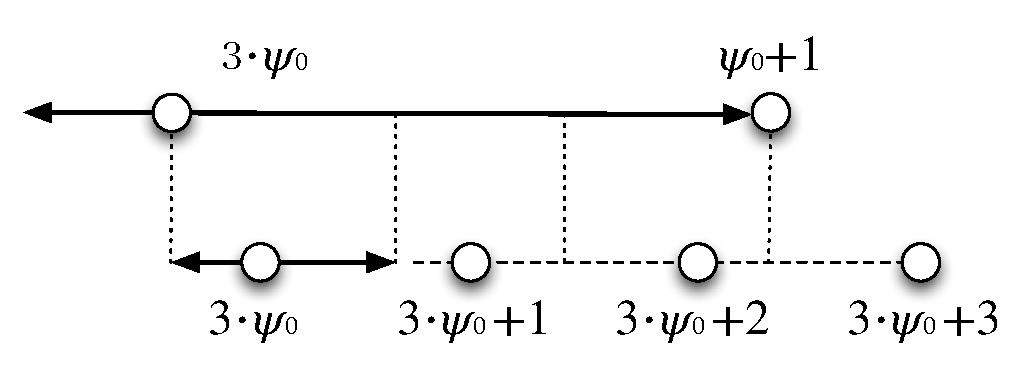
\includegraphics[width=0.5\linewidth]{images/constraintsup}
\caption{Timing diagram of upsampling}
\label{fig:constraintsup}
\end{figure}

We can relate the timing diagram to a waveform format often used for hardware simulation purposes, as shown in figure \ref{fig:ratechangetiming}.
This waveform format shows that the output sequence is constructed using $in$, $x$ and $y$.
This means that $in$ is ascribed with $3 \cdot \psi$, which is possible since we only ascribe $in$ with a \textit{more} restrictive time expression.
As the input in this example is only used for a single cycle we can deduce that, while the lifetime of $in$ could be from $\psi$ to $\psi+1$, for this example only a lifetime of $\psi$ to $3\cdot\psi+1$ is needed.

\begin{figure}[h]
\centering
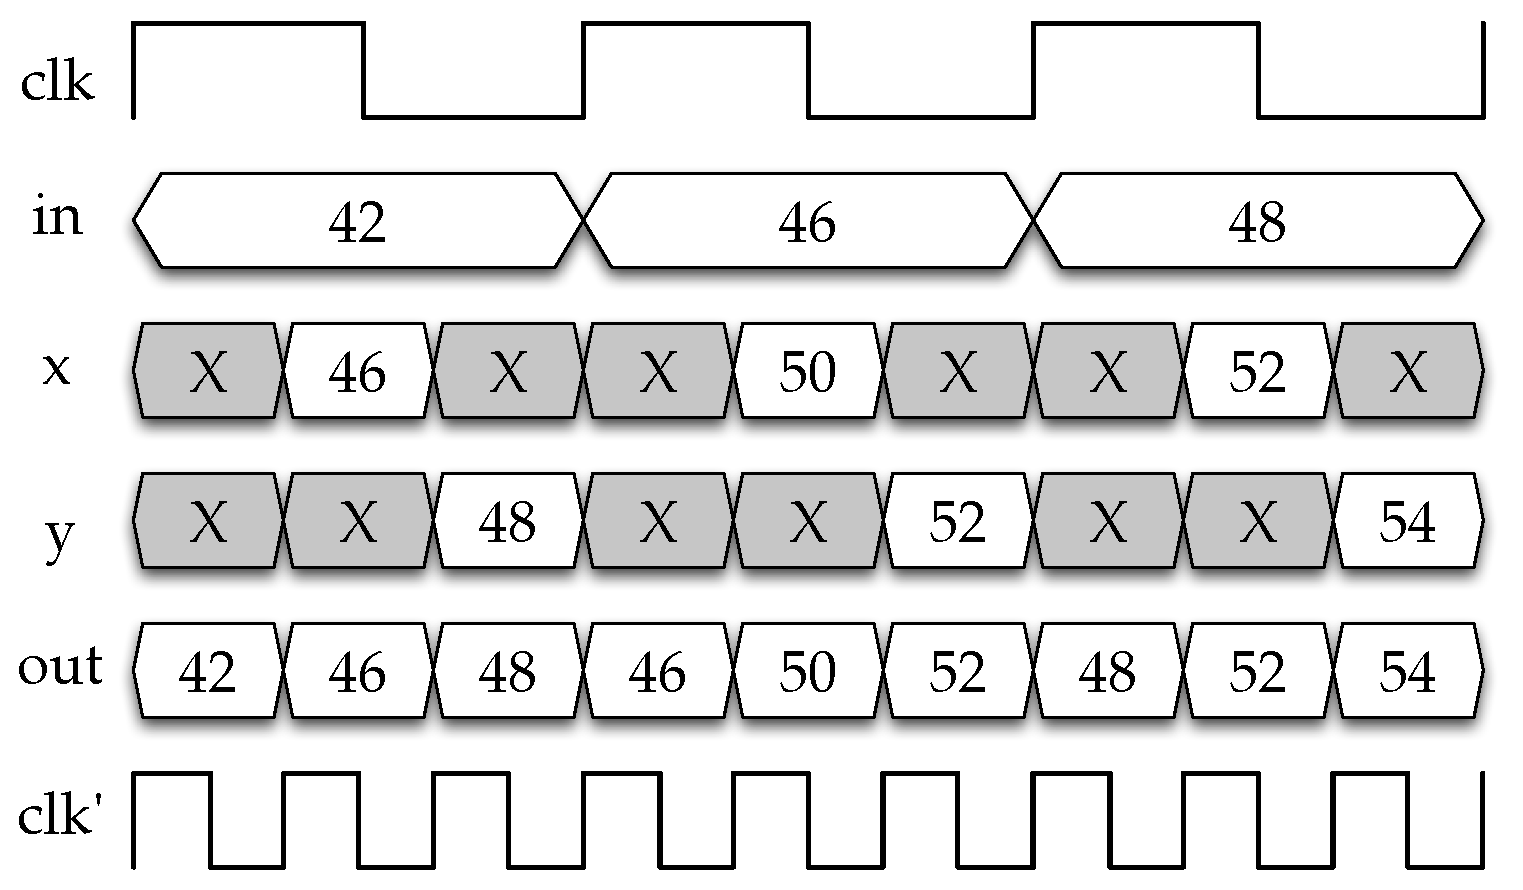
\includegraphics[width=0.7\textwidth]{images/ratechangetiming}
\caption{Example waveform of the circuit of figure \ref{fig:ratechange}}
\label{fig:ratechangetiming}
\end{figure}

When using rates we still have to take care of causality however.
Suppose we have the timing diagram of figure \ref{fig:constraintsup}, when we would want to downsample $3 \cdot \psi_0 + 1$ to $\psi$ we can only allow this if the result actually occurs at $\psi+1$, since $3 \cdot \psi + 1$ is strictly greater than $3 \cdot \psi$, which means that, by transivity $3 \cdot \psi + 1 > \psi$.
These constraints can be derived given the constraint $\psi \le 3 \cdot \psi$.

Upscaling and downscaling can also be done automatically. 
For instance, given the constraint $3 \cdot \psi \le 6 \cdot \psi$, we could upscale the values of the left hand side to the rate of the right hand side.
For this to work however, the rate used in the right hand side of the inequality has to be a multiple of the rate on the left hand side.
If we would allow non-multiples then we would not be sure when \textit{exactly} two moments in time occur in relation to each other.

While languages which use the streaming principle make streams first-class values, we do not do so here.
Whenever we create a sequence we are not allowed to refer to the sequence using a single variable.
This means that, when we create a sequence using multiple expressions as elements, we may only refer to the elements of the sequence, not the sequence in its entirety.

\subsubsection{Sampling and Mapping}
The sequencing operation offers some interesting possibilities when it comes to mapping a description to a stream of values.
As an example, we introduce the component of figure \ref{fig:summapc1}.

\begin{figure}[h]
\centering
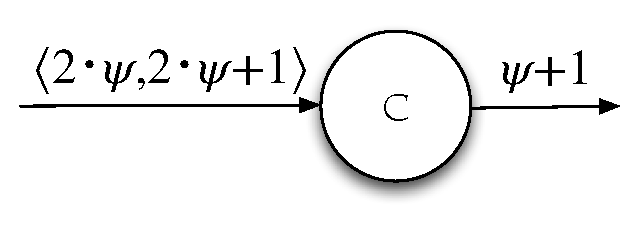
\includegraphics[width=0.4\textwidth]{images/summapc1}
\caption{Upsampling component}
\label{fig:summapc1}
\end{figure}

This downsamples the input. 
We can see from the timing diagram in figure \ref{summap1} that the output $\psi$ changes once when $2 \cdot \psi$ changes twice.
Suppose the component $C$ adds two subsequent values as in $C \langle x, y \rangle = x + y$.
When we supply this component with the input stream $0,1,2,3,4,5$ the result would be $1,5,9$, as both values of the input change when the output changes once.

\begin{figure}[h]
\centering
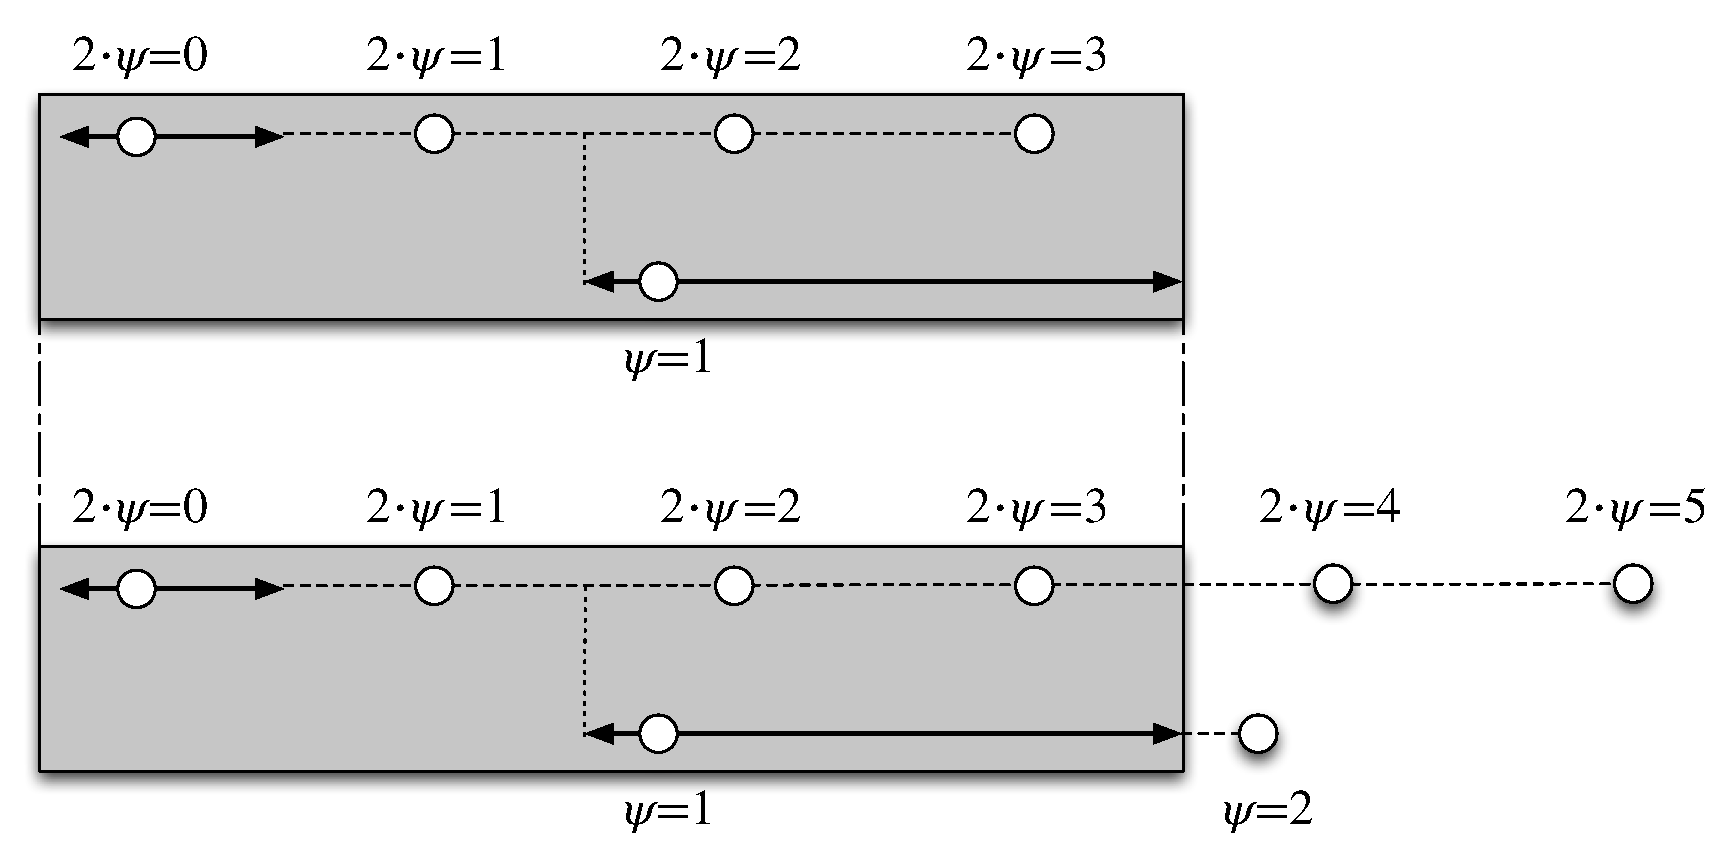
\includegraphics[width=\textwidth]{images/summap1}
\caption{Timing diagram of upsampling when mapped to a stream}
\label{fig:summap1}
\end{figure}

When the timing behaviour of the component is changed to the one shown by figure \ref{fig:summapc2} this changes however.

\begin{figure}[h]
\centering
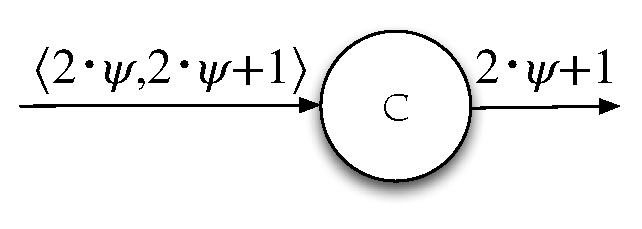
\includegraphics[width=0.4\textwidth]{images/summapc2}
\caption{Sampling operation in a component}
\label{fig:summapc2}
\end{figure}

This component does not downsample the input, yet it only defines a \textit{single} output, while the input defines two values.
As a result, when we take the same definition $C \langle x, y \rangle = x + y$ the input stream $0,1,2,3,4,5$ is transformed to $1,3,5,7,9$.

\begin{figure}[h]
\centering
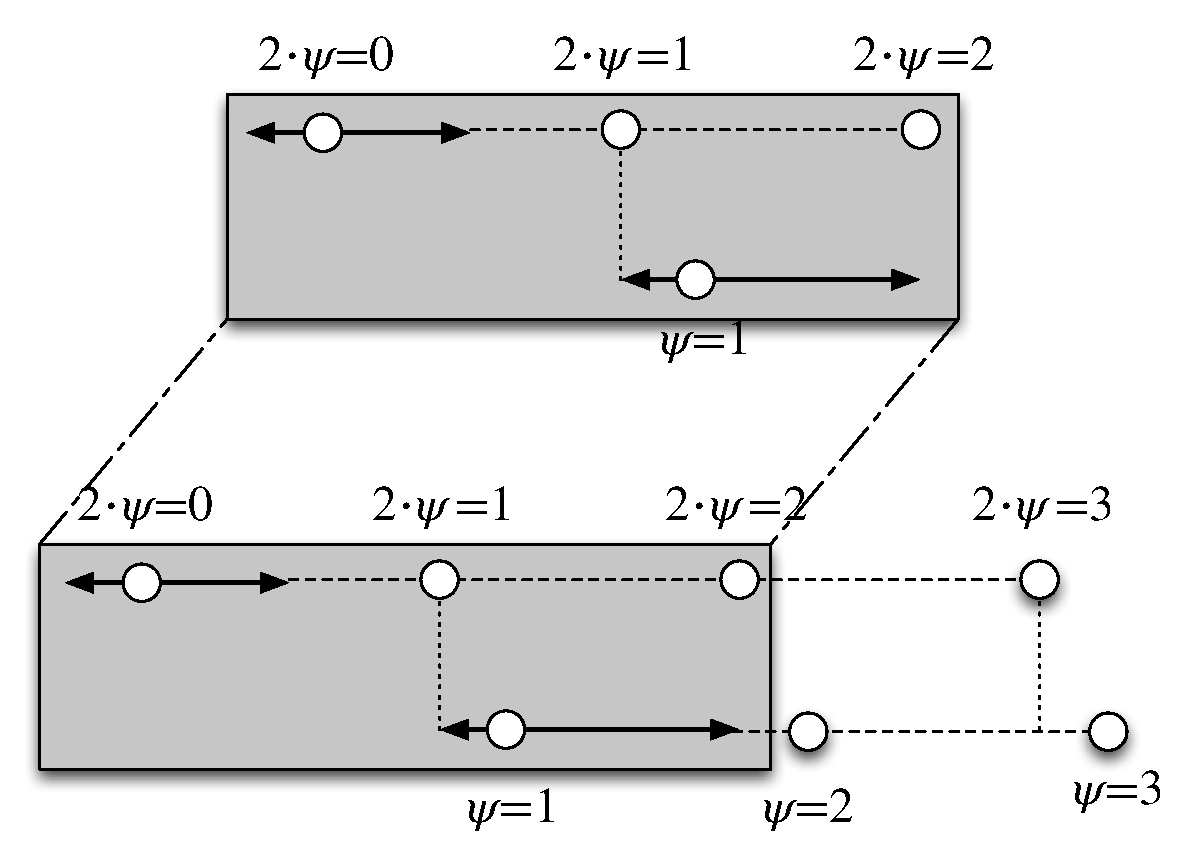
\includegraphics[width=0.7\textwidth]{images/summap2}
\caption{Timing diagram of sampling}
\label{fig:summap2}
\end{figure}

The differences between the two operations is that the former defines \textit{downsampling} while the second example introduces \textit{sampling} without changing the rate of change.
This shows that introducing a sequence allows us to define upsampling, downsampling as well as regular sampling.

\FloatBarrier
%%%%
% Informal Overview
%%%%
\subsection{Informal Overview}
The model of time we use is not unique, as we rely on discrete instances of time.
It has already been described by \citeauthor{lee1998framework} through the tagged event model, as explained in the previous chapter.
In this model every value is tagged with a timestamp and together they are called events.

Events by themselves cannot fully describe the behaviour of circuits.
While \citeauthor{lee1998framework} use signals to describe the entire behaviour of a component, we use abstract events and relations between abstract events to describe the timing behaviour of a circuit.
We only allow description of an abstract event in the sense that we only know the type of values and the lifetime of values in terms of the lifetime of other values.
The types of values can be known through constraint-based typing, while the lifetime of values can be known through our type-system, which we will formally introduce in the next section.
The types of values allows us to determine the amount of wires and memory elements to use, while the lifetime allows us to reason about the periodic behaviour of values.

The distinction between a signal and abstract event is important, as streaming languages allow variables to describe entire signals, and allow access to previous values from any given signal.
Here we only assume events and as such we do not have a notion of a previous value. 
While we have introduce the notion of a sequence, we never allow sequences to be first-class.

For our purposes, namely specifying the timing behavior of hardware designs, timing is considered uniform, at least when focussing on designs which use a single clock source.
As such, the problem of maintaining a consistent view of time as mentioned by \citeauthor{lee1998framework} is not an issue here, though it might introduce significant problems when considering multiple clock domains.

The model of time we introduces does not differ greatly from those used in synchronous languages.
In Esterel\cite{berry1992esterel} time is \textit{monitored} using watchdogs, triggers and temporal loops, without having the ability to \textit{specify} the timing tags directly.
The same can be said about Lustre and Signal.
In these languages timing \textit{emerges} from the specification as opposed to being part of the specification.
This is not the case here, as we define a specific event to occur at a specific time instance and it is up to the type checker to ensure our description is a correct representation of an actual circuit.
Behaviour still emerges from composition, as composition may change how two components interact.
However, once the component is defined to have a certain behavior, composition may only \textit{add} logic to ensure the composition behaves as intended.
In the next section we will formalize the semantics of our type-checking and inference rules through operational semantics.



\newpage
%%%%
% Formal Semantics
%%%%
\section{Formal Semantics}
As in the previous chapter when we introduced the simply typed $\lambda$-calculus, and constraint-based $\lambda$-calculus, we will introduce our typing rules using operational semantics.
We will completely ignore traditional types in our expressions and only define the timing behaviour described by our type-system.
Furthermore, we will first focus only on memory elements and combinational logic, without referring to rate-changes.

First, we will introduce the grammar of a modified form of the $\lambda$-calculus, which we will call $\lambda_\psi$.
After introducing the grammar we will define the relation between expressions of $\lambda_\psi$ to time expressions through typing rules.
When we have introduced the typing rules we will infer the timing behaviour of a trivial circuit in order to show that the typing rules we have defined behave sanely.
After doing so we introduce how we can upsample and downsample 
Later on we will introduce typing rules and extensions to our grammar named $\lambda_\psi$ to formalize rate-changes.


\subsection{The Grammar of $\lambda_\psi$}
As time variables are similar to type variables we will use $\tau,\sigma,\rho$ to range over time variables.
First we introduce the set of timing constraints $\mathcal{C}$, shown in definition \ref{def:constraintpsi} which express relations between time expressions.

\begin{definitiontitled}[text only,float]{Set of constraints $\mathcal{C}$}{def:constraintpsi}
Let $\tau$ and $\sigma$ be time expressions with associated rates $r$, $s$ and offsets $a$, $b$, then the $i^{th}$ \textbf{time-constraint} $\mathcal{C}_i$ is defined as an element of the set $\mathcal{C}$ as follows:
\[
\mathcal{C}   = \{\mathcal{C}_i | i \in 1..n\} \quad
\mathcal{C}_i = \left\{ 
  \begin{array}{l} 
  \tau \le \sigma = r \cdot \psi_\tau + a \le s \cdot \psi_\sigma + b \: | \: \exists d. \frac{s}{r} = d \\ 
  \tau = \sigma = r \cdot \psi_\tau + a = s \cdot \psi_\sigma + b\\ 
\end{array} \right.
\]
, where $\le$ is the non-strict ordering relation and $=$ is the equality relation.
The non-strict ordering relation $\le$ allows a change in rate \textit{only} when there exists a divisor $d$ such that $\frac{s}{r} = d$.
This means that $r$ must be a factor of $s$ in order for the relation to be valid.
\end{definitiontitled}

Similar to $\Gamma$, $\Delta$ provides a mapping between term variables of the $\lambda$-calculus and time variables, as per definition \ref{def:deltacontext}.
This context will provide us with the information we need when defining the operational semantics of our typing rules.

\begin{definitiontitled}[text only,float]{Timing Context $\Delta$}{def:deltacontext}
The \textbf{timing context} $\Delta$ is a set of bindings $x@\tau$, where $x$ is a variable representing a value and $\tau$ is the time expression bound to the variable.
\end{definitiontitled}

The context $\Delta$ is part of the grammar of our time-aware $\lambda$-calculus, $\lambda_\psi$, which is introduced in defition \ref{def:lambdapsi}.  
This grammar is based on the grammar of the constraint based $\lambda$-calculus introduced in the previous chapter.
Main differences include the \textbf{at} keyword, which is the temporal equivalent of the \textbf{as} keyword used for type ascription, the already introduced $\delta$ operation and time expressions, the $+$ operation and the time abstraction operator $\Psi$.
The $+$ operation is merely introduced to create more meaningful examples.

Timing expressions can be created using a multiplicant $r$ and an offset $a$.
These timing expressions only make sense when relations between them are created through abstraction and application.
To allow further specification, the \textbf{at} keyword can bind expressions to a specific time expression.
When we introduce a time variable through the $\Psi$ operation we can use multiple ascriptions and refer to the same time variable.
This allows us to manually constraint components in ways which are not possible using just the abstraction and application operations.
For instance, in the expression $\Psi \psi. \lambda x. \lambda y. (x \textbf{ at } \psi) + (y \textbf{ at } \psi + 1)$ we relate the input labelled $x$ to the input labelled $y$ such that $x$ occurs at $\psi$ and $y$ one clockcycle later. These two values from two distinct clockcycles are then added.

\begin{definitiontitled}[text only,float]{Grammar of $\lambda_\psi$}{def:lambdapsi}
\begin{changemargin}{-0.5cm}{0cm}
\begin{minipage}[b]{0.50\linewidth}
\begin{tabular}{lclr}
e       & $\Coloneqq$ &                 & expressions: \\
        & |    & x                     & (variable) \\
        & |    & $\lambda$x.e          & (abstraction) \\
        & |    & e e                   & (application) \\
        & |    & c                     & (constant) \\
        & |    & \textbf{let} x = e \textbf{in} e        & (let binding) \\
        & |    & e at $\tau$           & (ascription) \\
        & |    & $\delta$ e              & (strict delay) \\
        & |    & $\Psi$ $\psi$.e          & (time abstraction) \\
        & |    & e + e                  & (addition) \\
\end{tabular}
\end{minipage}
\begin{minipage}[b]{0.40\linewidth}
\begin{tabular}{lclr}
c       & $\Coloneqq$ &                & constants \\
        & |    & true                  & (Boolean true) \\
        & |    & false                 & (Boolean false) \\
        & |    & n $\in \mathbb{Z}$    & (Integer literals) \\
\\
$\tau$  & $\Coloneqq$ & $r \cdot \psi + a$    & (time expression) \\
$r$     & $\Coloneqq$ & $r \in \mathbb{N}_0$  & (rate) \\
$a$     & $\Coloneqq$ & $o \in \mathbb{N}_0$  & (offset) \\
\\
$\Delta$& $\Coloneqq$ &                 & contexts: \\
        & |     & $\emptyset$           & (empty context) \\
        & |     & $\Delta,x@\tau$       & (time binding). \\
\end{tabular}
\end{minipage}
\end{changemargin}
\end{definitiontitled}

\subsection{Typing Rules for Memory Elements}
Using this grammar we can then create typing rules, similar to the typing rules of constraint based type-checking in the previous chapter.
In constraint based typing terms are only well-typed when the constraints hold under unification.
Here, our constraints are subject to a modified form of unification, but for the purpose of specifying typing rules  we do not need to introduce it in detail.
Like earlier, the judgement $\Delta \vdash \lambda x.e @ \sigma | \mathcal{T} \: \mathcal{C}$ states that we may derive $\lambda x.e$ to produce a result at the time expressed by $\sigma$, under condition that the constraints using the time variables in $\mathcal{T}$ in $\mathcal{C}$ hold.

\begin{definitiontitled}[text only]{Typing Rules for $\lambda_\psi$}{def:typerulelambdapsi}
\begin{tabularx}{\textwidth}{ r r X r}
\centering
$ \displaystyle \frac{ x @ \sigma \in \Delta
}{      \Delta \vdash x @ \sigma |_\varnothing \: \{\}}
$ &
TT-Var
&
$ \displaystyle 
\frac{  \begin{array}{c}
          \Delta,x@\psi_0 \vdash e @ \tau \: |_\mathcal{T} \: \mathcal{C}\\
          \mathcal{C}' = \mathcal{C} \cup \{ \tau \le \psi_1, \psi_0 \le \psi_1 \}  \\
          unique(\psi_0, \psi_1, \tau, \mathcal{T}) \\
        \end{array}
} { \Delta \vdash \lambda x.e @ \psi_1 \: |_{\mathcal{T} \cup \psi_0 \cup \psi_1} \: \mathcal{C}'}
$ 
& TT-Abs \\
\\

& &
$ \displaystyle
\frac{  \begin{array}{c}
          \Delta \vdash e_1 @ \sigma \: |_{\mathcal{T}_1} \: \mathcal{C}_1 
            \quad \Delta \vdash e_2 @ \tau \: |_{\mathcal{T}_2} \: \mathcal{C}_2 \\
          \mathcal{C}' = \mathcal{C}_1 \cup \mathcal{C}_2 \cup \{\tau \le \psi, \sigma \le \psi \} \\
          unique(\psi, \sigma, \tau ,\mathcal{T}_1, \mathcal{T}_2) \\
        \end{array}
} { \Delta \vdash e_1 \: e_2 @ \psi \: |_{\mathcal{T}_1 \cup \mathcal{T}_2} \: \mathcal{C}' }
$ & TT-App \\
\\

$ \displaystyle
  \frac
    { c @ \sigma \in \Delta }
    { \Delta \vdash c @ \sigma |_\varnothing \: \{\}}
$
&
TT-Const
& 
\centering
$ \displaystyle
  \frac
  { \Delta \vdash [ x \mapsto e_1] e_2 @ \tau |_\mathcal{T} \: \mathcal{C} }
  { \Delta \vdash \textbf{let } x = e_1 \textbf{ in } e_2 @ \tau |_\mathcal{T} \: \mathcal{C}} 
$
&
TT-Let\\
\\

$ \displaystyle
  \frac
  { }
  {\Delta \vdash (+) @ \psi |_\mathcal{T} \: \{\}}
$
&
TT-Plus
&
\centering
$ \displaystyle
  \frac
  { \begin{array}{c}
      \Delta \vdash e @ \tau |_\mathcal{T} \: \mathcal{C}\\
      \mathcal{C}' = \mathcal{C} \cup \{\tau = \psi\}
    \end{array}
  }
  { \Delta \vdash \delta e @ \psi + 1 } 
$
& 
TT-Delta\\
\\

$ \displaystyle
  \frac
  { \Psi \psi.e }
  { \psi \in \Delta}
$
&
TT-Psi
&

\centering
$ \displaystyle \frac{  \begin{array}{c} 
                          \Delta \vdash e @ \tau \: |_\mathcal{T} \: \mathcal{C} \quad \sigma \in \Delta \\
                          \mathcal{C}' = \mathcal{C} \cup \{ \tau \le \sigma \}
                        \end{array}}
{ \Delta \vdash (e \text{ at } \sigma) @ \sigma \: |_\mathcal{T} \: \mathcal{C}' }
$
& TT-At
\\

\end{tabularx}
\end{definitiontitled}

The rules TT-Var and TT-Const have not changed much at all.
In fact, only the ``is-of-type'' operation $:$ has changed to $@$.
This is much different for the other rules, especially when we consider the TT-Abs rule.

To allow type-inference and automatic insertion of memory elements, the TT-Abs rule introduces two new time variables.
The $\lambda$-abstraction introduces a variable $x$. 
Without considering how $x$ is used in the expression $e$, which is the body of the function expressed by the abstraction, we do not know the constraints on the temporal behaviour of $x$.
Since we do not know anything we assign a \textit{fresh} time variable to $x$.
By fresh we mean that it is not used anywhere else in the context.
The expression $e$ in which $x$ is used must result in a value at some moment in time expressed by $\tau$.
Finally, the complete result of $\lambda x.e$ must result in a value at some moment in time $\psi_1$, which is also a fresh variable.
This is made more clear by the timing diagram of figure \ref{fig:ttabs}.

\begin{figure}[h]
\centering
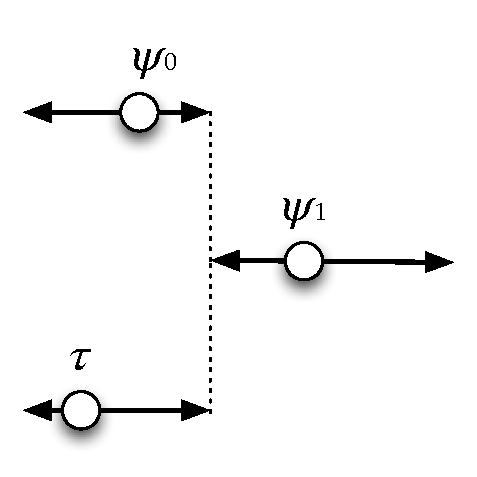
\includegraphics[width=0.2\textwidth]{images/ttabs}
\caption{Timing diagram of TT-Abs}
\label{fig:ttabs}
\end{figure}


Creating an independent time variable $\psi_1$ might seem redundant, as we already defined $e$ to result in a value as defined by $\tau$.
However, in an n-ary function we do not know what order the arguments are supplied without making claims about the context.
For instance, in $\lambda x. \lambda y. x + y$, we do not know if $\psi_x \le \psi_y$ or $\psi_y \le \psi_x$.
For this reason we introduce an extra variable $\psi_1$.
This does have the side-effect of being overly restrictive in the case of unused variables, such as in $\lambda x. \lambda y. y$.
Since $x$ is never used, we should not create any constraint between $x$ and $y$. 
This is only a minor issue however, as unused variables are not very realistic in practice.

The rule TT-App also introduces a time variable. 
In TT-App, the time expressions bound to $e_1$ and $e_2$ are restricted by some moment in time $\psi$, which is a fresh variable.
In regular type-checking, $e_1$ must always have a function type, but since we do not distinguish functions from other values, we never mention this in our typing rules.
When $e_1$ is available at $\sigma$ and $e_2$ at $\tau$ then, whenever we apply $e_1$ to $e_2$, the result must be available at $\psi$, with $\sigma \le \psi$ and $\tau \le \psi$.
This is clarified by the timing diagram of figure \ref{fig:ttapp}.

\begin{figure}[h]
\centering
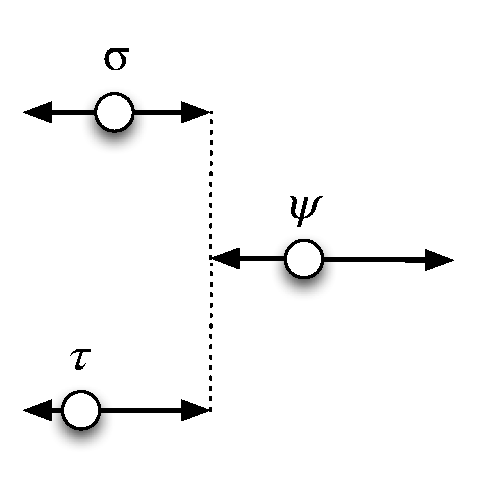
\includegraphics[width=0.2\textwidth]{images/ttapp}
\caption{Timing diagram of TT-App}
\label{fig:ttapp}
\end{figure}

The definition of TT-At is fairly straightforward.
We can delay values indefinitely if we so desire, which is what the TT-At rule expresses.
The TT-At rule allows ascription of expressions with time expressions.
As long as the time expression $\sigma$ the expression $e$ is ascribed with does not occur before $\tau$, which is the time expression of $e$ known from the context, then $e \textbf{ at } \sigma$ adds the constraint $\tau \le \sigma$.

TT-Let, like in constraint-based typing, performs a step of evalutation.
The step of evalutation effectively removes the let binding, allowing type checking as usual.
In practice this is not the most effective method, though that is mostly an implementation detail.
In chapter x\todo{ref}, when we cover the implementation of the prototype, we will go into further detail.

TT-Plus allows us to use the $+$ operation as if it were a block of combinational logic.
Whenever we encounter the $+$ operations we can always derive a time expression, under the condition that $\psi$ is fresh.
TT-Delta behaves as discussed earlier in the informal section. 
Through the equality operation the relation $\tau = \psi$ is introduced, after which we create a new time expression by defining the result $\delta.e$ to be available at $\psi + 1$.
Time variables may be introduced manually through the $\Psi$ operation, which merely places $\psi$ within $\delta$.

While we have defined the rules, it is hard to see how these rules may be used, or whether they are even correct.
In the next section we will use the typing rules of \ref{def:typerulelambdapsi} to infer the timing behaviour of a simple circuit.

\subsection{Inferring Time}
To show how we can use these rules to infer timing behaviour, we first introduce the (trivial) circuit of figure \ref{fig:addcomp}.
There, we have defined an adder with the intention of adding two registers within its definition.

\begin{figure}[h]
\centering
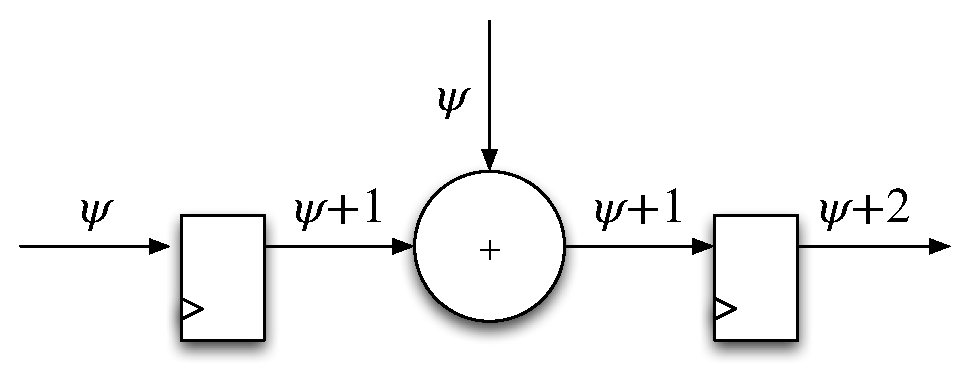
\includegraphics[width=0.8\linewidth]{images/addcomp}
\caption{An adder with two memory elements}
\label{fig:addcomp}
\end{figure}

Using the grammar of $\lambda_\psi$, we can create a term which represents this circuit as follows:
\begin{changemargin}{1cm}{0cm}
\begin{expansionno}{text only}
$
\begin{array}{l l l} 
\Psi \psi. \lambda x.\lambda y. & \textbf{let } & x' = x \textbf{ at } \psi\\ 
                                &     & y' = y \textbf{ at } \psi+1\\
                                & \textbf{in }  & x' + y' \textbf{ at } \psi + 2
\end{array}$
\end{expansionno}
\end{changemargin}

Since we have defined the let binding as performing a step of evaluation, when we remove the let-bindings we end up with the following expression:
\begin{changemargin}{1cm}{0cm}
\begin{expansionno}{text only}
$
\Psi \psi. (\lambda x.\lambda y. (x \textbf{ at } \psi) +  (y \textbf{ at } \psi+1) \textbf{ at } \psi + 2)
$
\end{expansionno}
\end{changemargin}


To simplify the derivation of time constraints we will first only derive $\lambda x. \lambda y. x + y$.
Afterwards we will selectively apply the TT-At rule to define at which places registers ought to be inserted.
Using the Gentzen style of natural deduction we derive $\lambda x. \lambda y. x + y$ as follows:
\begin{prooftree}
\rootAtTop
\def\extraVskip{8pt}
\AxiomC{}
  \RightLabel{TT-Plus (7)}
  \UnaryInfC{$\Delta \vdash +@\psi_+$}
    \AxiomC{$x \in \Delta$}
    \RightLabel{TT-Var (6)}
    \UnaryInfC{$\Delta \vdash x@\psi_x \in \Delta$}
  \RightLabel{TT-App (5)}
  \BinaryInfC{$\Delta \vdash + x @ \psi_3 | \mathcal{C}_0 = \{\psi_x \le \psi_3, \psi_+ \le \psi_3\}$}
    \AxiomC{$y \in \Delta$}
    \RightLabel{TT-Var (4)}
    \UnaryInfC{$\Delta \vdash y@\psi_y \in \Delta$}
  \RightLabel{TT-App (3)}
  \BinaryInfC{$\Delta \vdash + x y @ \psi_2 | \mathcal{C}_1 = \mathcal{C}_0 \cup \{\psi_y \le \psi_2, \psi_3 \le \psi_2 \}$}
\RightLabel{TT-Abs (2)}
\UnaryInfC{$\Delta,y@\psi_y \vdash \lambda y. + x y @ \psi_1 | \mathcal{C}_2 = \mathcal{C}_1 \cup \{\psi_y \le \psi_1, \psi_2 \le \psi_1 \} $}
\RightLabel{TT-Abs (1)}
\UnaryInfC{$\Delta,x@\psi_x \vdash \lambda x. \lambda y. + x y @ \psi_0 | \mathcal{C}_2 \cup \{\psi_x \le \psi_0, \psi_1 \le \psi_0 \} $}
\end{prooftree}

Using this derivation we have the following set of constraints:
\[
\begin{array}{l l l l l}
C_2 = & \{ & \psi_x \le \psi_0, & \psi_1 \le \psi_0 \\
      &,   & \psi_y \le \psi_1, & \psi_2 \le \psi_1 \\
      &,   & \psi_y \le \psi_2, & \psi_3 \le \psi_2\\
      &,   & \psi_x \le \psi_3, & \psi_+ \le \psi_3 & \} \\ 
\end{array}
\]
, which we can express in the time diagram of figure \ref{fig:addcomptime}.

\begin{figure}[h]
\centering
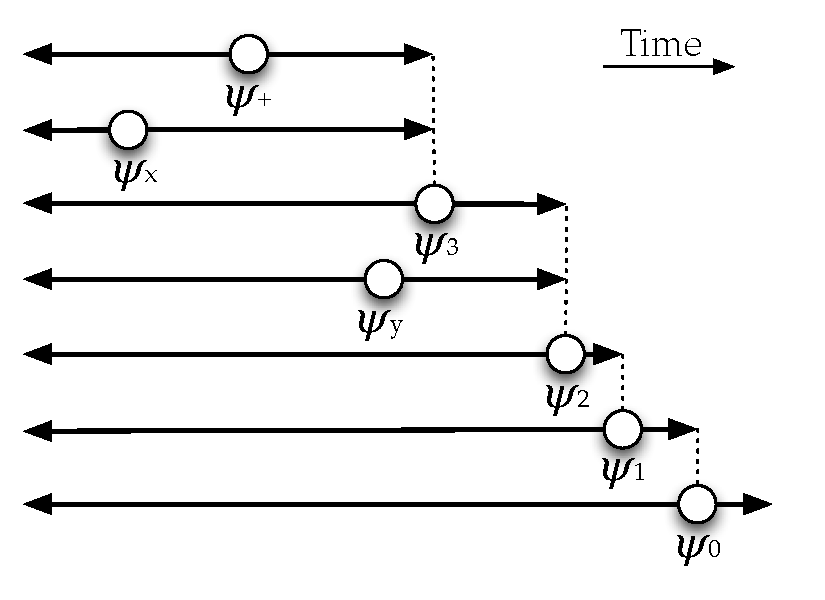
\includegraphics[width=0.6\linewidth]{images/addcomptime}
\caption{Constraints of the inferred timing of the circuit in figure \ref{fig:addcomp}}
\label{fig:addcomptime}
\end{figure}

These constraints by themselves are meaningless, as we only derived the ordering in execution.
However, we can add the TT-At statements to introduce the constraints $\psi_x \le \psi$, $\psi_y \le \psi+1$ and $\psi_0 \le \psi+2$.
While we do not derive these statements here, we can see that, aside from adding these constraints we also have to rewrite the other set of constraints.
For instance, in the rule TT-App (3), when we would insert the TT-At rule $\psi_y$ would be replaced by $\psi+1$, which changes the constraint introduced by TT-App (3) from $\psi_y \le \psi_2$ to $\psi + 1 \le \psi_2$.
To clarify we have shown part of the derivation including the TT-At rule below.
\begin{prooftree}
\rootAtTop
\def\extraVskip{8pt}
\AxiomC{$\Delta \vdash + x @ \psi_3 \ldots$}
\AxiomC{$\Delta \vdash y@\psi_y \: |_\varnothing \: \{\}$}
\RightLabel{TT-At (a)}
\UnaryInfC{$\Delta \vdash y \textbf{ at } \psi + 1@\psi + 1 |_\varnothing \: \{\psi_y \le \psi + 1\}$}
\RightLabel{TT-App (3)}
\BinaryInfC{$\Delta \vdash + x y @ \psi_2 | \mathcal{C}_1 = \mathcal{C}_0 \cup \{\psi + 1 \le \psi_2, \psi_3 \le \psi_2 \}$}
\end{prooftree}


When we replace these we obtain the following set of constraints:

\[
\begin{array}{l l l l l}
C_2 = & \{ & \psi_x \le \psi_0, & \psi_1 \le \psi_0 \\
      &,   & \psi_y \le \psi_1, & \psi_2 \le \psi_1 \\
      &,   & \psi + 1 \le \psi_2, & \psi_3 \le \psi_2\\
      &,   & \psi \le \psi_3, & \psi_+ \le \psi_3 & \\ 
      &,   & \psi_x \le \psi, & \psi_y \le \psi + 1 \\
      &,   & \psi_0 \le \psi+2 & \}
\end{array}
\], which are hard to read.
The timing diagram of figure \ref{fig:addcomptime} uses these constraints however and shows a far more restricted behavior of our expression.
In the timing diagram we placed $\psi_y$ between $\psi$ and $\psi + 1$.
This means that, as $y$ is already delayed one cycle when compared to $x$, we do not have to add a memory element here; the context has provided the memory element already.
The output is available at $\psi_0$, which has a lower bound of $\psi_y$ through $\psi_1$ and $\psi_2$ and an upper bound through $\psi+2$.
To make the result of $x + y @ \psi_3$ available for $\psi_2, \psi_1, \psi_0$, we must use a memory element as well.

\begin{figure}[h]
\centering
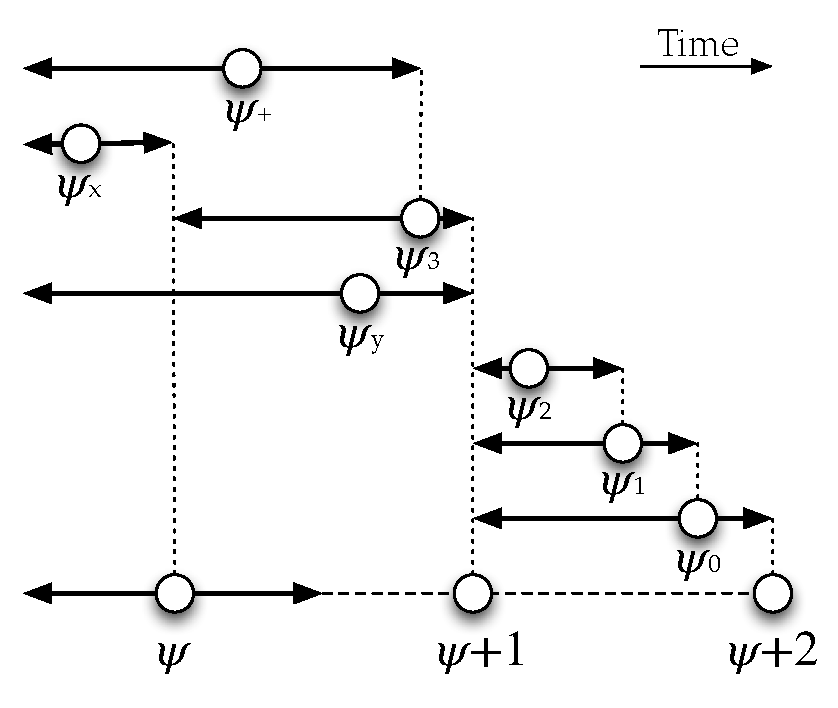
\includegraphics[width=0.6\linewidth]{images/addcomptime2}
\caption{Rewritten timing diagram of the circuit of figure \ref{fig:addcomp}}
\label{fig:addcomptime2}
\end{figure}

Through this derivation we have shown that we can indeed derive where memory elements need to be inserted, even though placement has only been done informally so far.
Later in this chapter we will modify the unification algorithm to formalise placement of memory elements.
Here, we have not fixed placement of memory elements.
For instance, in this derivation the argument named $y$ could be supplied at both $\psi$ as well as $\psi+1$, as both result in satisfied constraints.
This makes our definitions flexible and allows us to merely state the expected behaviour of circuits, without overly constricting ourselves with where memory elements ought to be inserted.

\subsection{Sequences in $\lambda_\psi$.}
To allow upscaling we first need to extend the grammar of definition \ref{def:lambdapsi} to allow sequences of values.
Sequences of values are like lists in that the number of elements can vary.
Unlike lists however, sequences are always finite.
Using the notation $\langle e_1, e_2, \ldots e_n \rangle$ we can create a sequence with $n-1$ elements.
Sequences ensure that $e_1$ occurs before $e_2$, $e_2$ before $e_3$, et cetera.
We have extended the definition of \ref{def:lambdapsi} below.

\begin{definitiontitled}[text only]{$\lambda_\psi$}{def:lambdapsi2}
\begin{tabular}{lclr}
$\Delta$& $\Coloneqq$ & $\Delta,\langle e, e, \ldots, e \rangle @s$ & (sequence binding) \\
          & |         & $\ldots$ \\
\\
$e$     & $\Coloneqq$ &  $\langle e, e, \ldots, e \rangle$ & (sequence expression) \\
        & |           &  $\ldots$ \\
\\
$s$     & $\Coloneqq$ & $\langle n \cdot \psi + i \: i = 0,1,\ldots,(n-1) \rangle$ & (time sequence)\\
\\
\end{tabular}
\end{definitiontitled}

What is noticable about this definition is the absence of an update to the timing expression $\tau$.
Since we consider sequences to not be first class, we can never use them in abstractions.
This severely limits the usage of sequences.
In the next chapter we will use syntactic sugar to allow sequences of values to be used in abstractions, without adding more rules to our type system.
Sequence expressions are associated with time expressions through the sequence binding in $\delta$.

\todo[inline]{In het volgende hoofdstuk ga ik in op hoe een functie een sequence kan accepteren dmv syntactic sugar.
Omdat we weten hoeveel elementen er in een sequence zitten kunnen we van een functie als f <x,y,z> = z , f x y z = z maken.
Omdat (toevallig!) in de typing rules geen rekening wordt gehouden met variabelen die niet gebruikt worden kan automatisch ook de juiste constraints op x,y,z worden afgeleid!}

However, we do need to show the relation between the expression $\langle e, e, \ldots, e \rangle$ and $s$, which we will do below.
\begin{definitiontitled}[text only]{Typing Rules for $\lambda_\psi$ (2)}{def:typepsi2}
\begin{tabularx}{\textwidth}{X r}
\centering
$ \displaystyle
  \frac{  \begin{array}{c}
            \Delta \vdash e_1 @ \tau |_\mathcal{T} \: \mathcal{C}, \ldots, \Delta \vdash e_n @ \sigma |_\mathcal{T} \: \mathcal{C}\\
            \mathcal{C}' = \mathcal{C} \cup \{ \tau = n \cdot \psi, \ldots, \sigma = n \cdot \psi + (n-1) \} 
          \end{array}}
  {\Delta \vdash \langle e_1, \ldots,  e_n \rangle @ \langle n \cdot \psi, \ldots, n \cdot \psi + (n-1) \rangle |_{\mathcal{T} \cup \psi} \: \mathcal{C}'}
$
& 
TT-Seq\\
\\

\centering
$ \displaystyle
  \frac{  \Delta \vdash \langle e_1, \ldots, e_n \rangle @ \langle n \cdot \psi, n \cdot \psi + (n-1) \rangle |_\mathcal{T} \: \mathcal{C}}
  {\Delta \vdash e_1@n \cdot \psi,\ldots, e_n @ n \cdot \psi + n |_{\mathcal{T}} \: \mathcal{C}}
$
&
TT-USeq\\
\\
\end{tabularx}
\end{definitiontitled}

These rules might seem complex, but they merely formalise the relation between the usage of a sequence in time expressions and term expressions.
In the rule TT-Seq we define $n-1$ expressions, named $e_1 \ldots e_n$. 
Since we are defining a sequence with values available at regular intervals we can forgo explicitly naming any expression in between $e_1$ and $e_n$ and focus only on the first and last element of the sequence.
This does not mean the elements in between $e_1$ and $e_n$ are ignored; the constraints to which these elements of the sequence are subject to are indeed added.
When we define a sequence of two elements, using $e_1$ and $e_2$, then $n = 2$, so the resulting sequence would have the associated time expression $\langle 2 \cdot \psi, 2 \cdot \psi + 1\rangle$.
This expresses that the resulting sequence changes at a rate which is twice as fast as $e_1$ and $e_2$ individually.
The rule TT-USeq is the inverse of TT-Seq and allows us to extract individual elements of a sequence.
Each individual element of the sequence retains the associated time expression.

\subsection{Feedback}
So far we have not mentioned feedback, which is essential to any serious hardware description language.
Figure \ref{fig:feedbacktime} shows feedback in the form of a mealy-machine.
From it we can see there is a conflict if $C$ represents combinational logic, as the $\psi + 1 \neq \psi$.
Even if we were to resolve that issue we still would not have a proper circuit, as the memory element needs to be initialized.
Without initialization we do not know what value the memory element contains when actual hardware is powered up.
This undefined value is maintained no matter what operations we perform on it, which means that due to the feedback loop this circuit would never result in a well-defined value.

\begin{figure}[h]
\centering
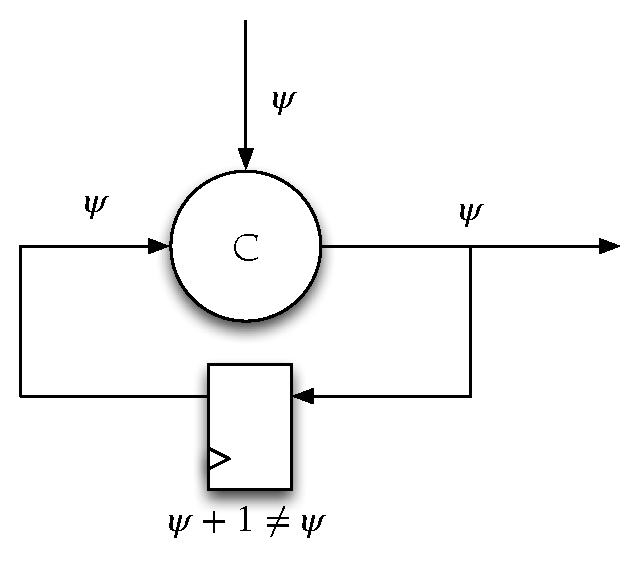
\includegraphics[width=0.5\linewidth]{images/feedback}
\caption{A timed adder with the constraints $(\psi_0,\psi_1) \le \psi_2$}
\label{fig:feedbacktime}
\end{figure}

To remedy this situation we use constant time moments to indicate initial values of memory elements.
For instance, when a value is defined at the constant time $0$, this means that this value is available when the circuit activates.
Since we already introduced sequences we can describe initialization followed by cyclic behaviour through sequences as well.
Given a time expression such as $\langle 0,1,\psi \rangle$ we can reason that the variable this expression is associated with has specific behaviour for cycles $0$ and $1$.
The remaining behaviour can be explained using $\psi$.

To formalise this understanding we first update the grammar of $\lambda_\psi$ to allow constants in sequences, shown in definition \ref{def:lambdapsi3}.

\begin{definitiontitled}[text only]{TT-Seq}{def:lambdapsi3}
\begin{tabular}{lclr}
$s$     & $\Coloneqq$ & $\langle n \cdot \psi + i \quad i = 0,1,\ldots,(n-1) \rangle$ & (time sequence)\\
        & |           & $\langle 0, 1, \ldots (n-1), n \cdot \psi + i \quad i = n,n+1,\ldots,2n-1 \rangle$ & (init sequence)\\
\end{tabular}
\end{definitiontitled}

From this definition we can see that the number of constants is equal to the number of time variables in the sequence.
This is a restriction in order to not further complicate the type-system.
If we were to allow it we would have to show exactly how constants relate to time variables.
Now we can reason that if $\psi_0 = 0$, then $\psi_0 < n \cdot \psi$ in $\langle 0, n \cdot \psi \rangle$. 

As an example, consider the following expression:
\begin{changemargin}{1cm}{0cm}
\begin{expansionno}{text only}
$
\begin{array}{l l l} 
\Psi \psi. \lambda x. & \textbf{let } & y = (42 \textbf{ at } 0)\\
                      &               & z = z + (x \textbf{ at } \psi) \\
& \textbf{in } & \langle y, z \rangle \\
\end{array}$
.
\end{expansionno}
\end{changemargin}
This expression has the associated time expression $\langle 0, \psi \rangle$.
Through the usage of the constant $y$ in the sequence $\langle y, z \rangle$ we allow the recursive definition of $z$.
When we associate $x$ with $\psi$, then without additional constraints we can also associate $z$ with $\psi$.
Since $z$ is used in the sequence of $\langle y, z \rangle$, we know that $y \le \psi - 1$.
Through this we can resolve the feedback operation, where $y$ represents the initial value of the register and $z$ expresses the combinational part of the feedback construction.
This means that feedback is caused by using constants in an expression, together with a time variable and by creating a recursive expression.

\subsection{Checking Time Constraints}
We have not formalised checking timing constraints.
Due to the fact that we allow the system to insert memory elements wherever they are needed, we cannot use straightforwared unification.
Given a set of timing constraints, we use SAT-solvers to verify whether our constraints hold.
However, to not completely forgo on proving that our type-system behaves sanely, we will check whether the constraints of the circuit of figure \ref{fig:addcomp} hold.
Since we do not have to add memory elements aside from the ones instructed via ascription, we do not need SAT-solvers to find a proper representation for this circuit to be able to verify it.
For this, we will use unification, which is partly re-introduced in pseudo-code below.

%% ODER: format ==         = "\mathrel{==}"
%% ODER: format /=         = "\neq "
%
%
\makeatletter
\@ifundefined{lhs2tex.lhs2tex.sty.read}%
  {\@namedef{lhs2tex.lhs2tex.sty.read}{}%
   \newcommand\SkipToFmtEnd{}%
   \newcommand\EndFmtInput{}%
   \long\def\SkipToFmtEnd#1\EndFmtInput{}%
  }\SkipToFmtEnd

\newcommand\ReadOnlyOnce[1]{\@ifundefined{#1}{\@namedef{#1}{}}\SkipToFmtEnd}
\DeclareFontFamily{OT1}{cmtex}{}
\DeclareFontShape{OT1}{cmtex}{m}{n}
  {<5><6><7><8>cmtex8
   <9>cmtex9
   <10><10.95><12><14.4><17.28><20.74><24.88>cmtex10}{}
\DeclareFontShape{OT1}{cmtex}{m}{it}
  {<-> ssub * cmtt/m/it}{}
\newcommand{\texfamily}{\fontfamily{cmtex}\selectfont}
\DeclareFontShape{OT1}{cmtt}{bx}{n}
  {<5><6><7><8>cmtt8
   <9>cmbtt9
   <10><10.95><12><14.4><17.28><20.74><24.88>cmbtt10}{}
\DeclareFontShape{OT1}{cmtex}{bx}{n}
  {<-> ssub * cmtt/bx/n}{}
\newcommand{\tex}[1]{\text{\texfamily#1}}	% NEU

\newcommand{\Sp}{\hskip.33334em\relax}


\newcommand{\Conid}[1]{\mathit{#1}}
\newcommand{\Varid}[1]{\mathit{#1}}
\newcommand{\anonymous}{\kern0.06em \vbox{\hrule\@width.5em}}
\newcommand{\plus}{\mathbin{+\!\!\!+}}
\newcommand{\bind}{\mathbin{>\!\!\!>\mkern-6.7mu=}}
\newcommand{\rbind}{\mathbin{=\mkern-6.7mu<\!\!\!<}}% suggested by Neil Mitchell
\newcommand{\sequ}{\mathbin{>\!\!\!>}}
\renewcommand{\leq}{\leqslant}
\renewcommand{\geq}{\geqslant}

%mathindent has to be defined
\@ifundefined{mathindent}%
  {\newdimen\mathindent\mathindent\leftmargini}%
  {}%

\def\resethooks{%
  \global\let\SaveRestoreHook\empty
  \global\let\ColumnHook\empty}
\newcommand*{\savecolumns}[1][default]%
  {\g@addto@macro\SaveRestoreHook{\savecolumns[#1]}}
\newcommand*{\restorecolumns}[1][default]%
  {\g@addto@macro\SaveRestoreHook{\restorecolumns[#1]}}
\newcommand*{\aligncolumn}[2]%
  {\g@addto@macro\ColumnHook{\column{#1}{#2}}}

\resethooks

\newcommand{\onelinecommentchars}{\quad-{}- }
\newcommand{\commentbeginchars}{\enskip\{-}
\newcommand{\commentendchars}{-\}\enskip}

\newcommand{\visiblecomments}{%
  \let\onelinecomment=\onelinecommentchars
  \let\commentbegin=\commentbeginchars
  \let\commentend=\commentendchars}

\newcommand{\invisiblecomments}{%
  \let\onelinecomment=\empty
  \let\commentbegin=\empty
  \let\commentend=\empty}

\visiblecomments

\newlength{\blanklineskip}
\setlength{\blanklineskip}{0.66084ex}

\newcommand{\hsindent}[1]{\quad}% default is fixed indentation
\let\hspre\empty
\let\hspost\empty
\newcommand{\NB}{\textbf{NB}}
\newcommand{\Todo}[1]{$\langle$\textbf{To do:}~#1$\rangle$}

\EndFmtInput
\makeatother
%
%
%
%
%
%
% This package provides two environments suitable to take the place
% of hscode, called "plainhscode" and "arrayhscode". 
%
% The plain environment surrounds each code block by vertical space,
% and it uses \abovedisplayskip and \belowdisplayskip to get spacing
% similar to formulas. Note that if these dimensions are changed,
% the spacing around displayed math formulas changes as well.
% All code is indented using \leftskip.
%
% Changed 19.08.2004 to reflect changes in colorcode. Should work with
% CodeGroup.sty.
%
\ReadOnlyOnce{polycode.fmt}%
\makeatletter

\newcommand{\hsnewpar}[1]%
  {{\parskip=0pt\parindent=0pt\par\vskip #1\noindent}}

% can be used, for instance, to redefine the code size, by setting the
% command to \small or something alike
\newcommand{\hscodestyle}{}

% The command \sethscode can be used to switch the code formatting
% behaviour by mapping the hscode environment in the subst directive
% to a new LaTeX environment.

\newcommand{\sethscode}[1]%
  {\expandafter\let\expandafter\hscode\csname #1\endcsname
   \expandafter\let\expandafter\endhscode\csname end#1\endcsname}

% "compatibility" mode restores the non-polycode.fmt layout.

\newenvironment{compathscode}%
  {\par\noindent
   \advance\leftskip\mathindent
   \hscodestyle
   \let\\=\@normalcr
   \let\hspre\(\let\hspost\)%
   \pboxed}%
  {\endpboxed\)%
   \par\noindent
   \ignorespacesafterend}

\newcommand{\compaths}{\sethscode{compathscode}}

% "plain" mode is the proposed default.
% It should now work with \centering.
% This required some changes. The old version
% is still available for reference as oldplainhscode.

\newenvironment{plainhscode}%
  {\hsnewpar\abovedisplayskip
   \advance\leftskip\mathindent
   \hscodestyle
   \let\hspre\(\let\hspost\)%
   \pboxed}%
  {\endpboxed%
   \hsnewpar\belowdisplayskip
   \ignorespacesafterend}

\newenvironment{oldplainhscode}%
  {\hsnewpar\abovedisplayskip
   \advance\leftskip\mathindent
   \hscodestyle
   \let\\=\@normalcr
   \(\pboxed}%
  {\endpboxed\)%
   \hsnewpar\belowdisplayskip
   \ignorespacesafterend}

% Here, we make plainhscode the default environment.

\newcommand{\plainhs}{\sethscode{plainhscode}}
\newcommand{\oldplainhs}{\sethscode{oldplainhscode}}
\plainhs

% The arrayhscode is like plain, but makes use of polytable's
% parray environment which disallows page breaks in code blocks.

\newenvironment{arrayhscode}%
  {\hsnewpar\abovedisplayskip
   \advance\leftskip\mathindent
   \hscodestyle
   \let\\=\@normalcr
   \(\parray}%
  {\endparray\)%
   \hsnewpar\belowdisplayskip
   \ignorespacesafterend}

\newcommand{\arrayhs}{\sethscode{arrayhscode}}

% The mathhscode environment also makes use of polytable's parray 
% environment. It is supposed to be used only inside math mode 
% (I used it to typeset the type rules in my thesis).

\newenvironment{mathhscode}%
  {\parray}{\endparray}

\newcommand{\mathhs}{\sethscode{mathhscode}}

% texths is similar to mathhs, but works in text mode.

\newenvironment{texthscode}%
  {\(\parray}{\endparray\)}

\newcommand{\texths}{\sethscode{texthscode}}

% The framed environment places code in a framed box.

\def\codeframewidth{\arrayrulewidth}

\newenvironment{framedhscode}%
  {\parskip=\abovedisplayskip\par\noindent
   \hscodestyle
   \arrayrulewidth=\codeframewidth
   \tabular{@{}|p{\linewidth-2\arraycolsep-2\arrayrulewidth-2pt}|@{}}%
   \hline\framedhslinecorrect\\{-1.5ex}%
   \let\endoflinesave=\\
   \let\\=\@normalcr
   \(\pboxed}%
  {\endpboxed\)%
   \framedhslinecorrect\endoflinesave{.5ex}\hline
   \endtabular
   \parskip=\belowdisplayskip\par\noindent
   \ignorespacesafterend}

\newcommand{\framedhslinecorrect}[2]%
  {#1[#2]}

\newcommand{\framedhs}{\sethscode{framedhscode}}

% The inlinehscode environment is an experimental environment
% that can be used to typeset displayed code inline.

\newenvironment{inlinehscode}%
  {\(\def\column##1##2{}%
   \let\>\undefined\let\<\undefined\let\\\undefined
   \newcommand\>[1][]{}\newcommand\<[1][]{}\newcommand\\[1][]{}%
   \def\fromto##1##2##3{##3}%
   \def\nextline{}}{\) }%

\newcommand{\inlinehs}{\sethscode{inlinehscode}}

% The joincode environment is a separate environment that
% can be used to surround and thereby connect multiple code
% blocks.

\newenvironment{joincode}%
  {\let\orighscode=\hscode
   \let\origendhscode=\endhscode
   \def\endhscode{\def\hscode{\endgroup\def\@currenvir{hscode}\\}\begingroup}
   %\let\SaveRestoreHook=\empty
   %\let\ColumnHook=\empty
   %\let\resethooks=\empty
   \orighscode\def\hscode{\endgroup\def\@currenvir{hscode}}}%
  {\origendhscode
   \global\let\hscode=\orighscode
   \global\let\endhscode=\origendhscode}%

\makeatother
\EndFmtInput
%

\begin{changemargin}{1cm}{0cm}
\begin{expansionno}{text only}
\begin{hscode}\SaveRestoreHook
\column{B}{@{}>{\hspre}l<{\hspost}@{}}%
\column{3}{@{}>{\hspre}l<{\hspost}@{}}%
\column{15}{@{}>{\hspre}l<{\hspost}@{}}%
\column{19}{@{}>{\hspre}l<{\hspost}@{}}%
\column{23}{@{}>{\hspre}l<{\hspost}@{}}%
\column{E}{@{}>{\hspre}l<{\hspost}@{}}%
\>[B]{}\Varid{unify}\;[\mskip1.5mu \mskip1.5mu]{}\<[15]%
\>[15]{}\mathrel{=}[\mskip1.5mu \mskip1.5mu]{}\<[E]%
\\
\>[B]{}\Varid{unify}\;(\tau\leq \sigma\mathbin{:}\mathcal{C}){}\<[E]%
\\
\>[B]{}\hsindent{3}{}\<[3]%
\>[3]{}\mid \tau\equiv \sigma{}\<[15]%
\>[15]{}\mathrel{=}{}\<[19]%
\>[19]{}\Varid{unify}\;\mathcal{C}{}\<[E]%
\\
\>[B]{}\hsindent{3}{}\<[3]%
\>[3]{}\mid \tau\equiv \psi\;\Varid{and}\;\psi\notin\Conid{FV}\;(\sigma){}\<[E]%
\\
\>[3]{}\hsindent{12}{}\<[15]%
\>[15]{}\mathrel{=}{}\<[19]%
\>[19]{}\mathbf{let}\;\Conid{C'}\mathrel{=}[\mskip1.5mu \tau\mapsto\sigma\mskip1.5mu]\;\mathcal{C}{}\<[E]%
\\
\>[19]{}\mathbf{in}\;{}\<[23]%
\>[23]{}[\mskip1.5mu \tau\mapsto\sigma\mskip1.5mu]\mathbin{:}(\Varid{unify}\;\Conid{C'}){}\<[E]%
\\
\>[B]{}\hsindent{3}{}\<[3]%
\>[3]{}\mid \sigma\equiv \psi\;\Varid{and}\;\psi\notin\Conid{FV}\;(\sigma){}\<[E]%
\\
\>[3]{}\hsindent{12}{}\<[15]%
\>[15]{}\mathrel{=}{}\<[19]%
\>[19]{}\mathbf{let}\;\Conid{C'}\mathrel{=}[\mskip1.5mu \sigma\mapsto\tau\mskip1.5mu]\;\mathcal{C}{}\<[E]%
\\
\>[19]{}\mathbf{in}\;{}\<[23]%
\>[23]{}[\mskip1.5mu \sigma\mapsto\tau\mskip1.5mu]\mathbin{:}(\Varid{unify}\;\Conid{C'}){}\<[E]%
\\
\>[B]{}\hsindent{3}{}\<[3]%
\>[3]{}\mid \Varid{otherwise}\mathrel{=}{}\<[19]%
\>[19]{}\Varid{error}\;\text{\tt \char34 Not~well-typed\char34}{}\<[E]%
\ColumnHook
\end{hscode}\resethooks
\end{expansionno}
\end{changemargin}




Expressed in the unification algorithm is the ordering relation.
We can distinguish between \textit{user-defined} time expressions and time expressions inserted through abstraction and application.
User-defined time expressions are the only ones, aside from the $\delta$ operator, which can insert offsets and rates.
To minimize the set of constraints, we replace all time variables with time expressions.
Since we use a ordering relation in our constraints we can unify our expressions in a fixed order, starting from the last-most (temporally speaking) constraint.

Given the following set of constraints, inferred from the circuit of figure \ref{fig:addcomp}, we will minimize the set of constraints.
\[
\begin{array}{l l l l l}
C_2 = & \{ & \psi_x \le \psi_0, & \psi_1 \le \psi_0 \\
      &,   & \psi_y \le \psi_1, & \psi_2 \le \psi_1 \\
      &,   & \psi + 1 \le \psi_2, & \psi_3 \le \psi_2\\
      &,   & \psi \le \psi_3, & \psi_+ \le \psi_3 & \\ 
      &,   & \psi_x \le \psi, & \psi_y \le \psi + 1 \\
      &,   & \psi_0 \le \psi+2 & \}
\end{array}
\]

First, we find a variable which does not occur on the left-hand side of the inequalities.
This means that, from a structural point of view, we start at the ``back'' of the circuit, rewriting time expressions as we move forward.
In the constraints above $\psi+2$ never occurs on the left hand side of the constraints, which means $\psi+2$ is unrestricted.
Following this, we substitute $[\psi_0 \mapsto \psi + 2]$, and remove duplicate expressions.

\[
\begin{array}{l l l l l}
C_2 = & \{ & \psi_x \le \psi + 2, & \psi_1 \le \psi + 2 \\
      &,   & \psi_y \le \psi_1, & \psi_2 \le \psi_1 \\
      &,   & \psi + 1 \le \psi_2, & \psi_3 \le \psi_2\\
      &,   & \psi \le \psi_3, & \psi_+ \le \psi_3 & \\ 
      &,   & \psi_x \le \psi, & \psi_y \le \psi + 1 \}
\end{array}
\]

Similarly we can replace $\psi_1$ with $\psi + 2$, and $\psi_2$ with $\psi + 2$, which were restricted by $\psi_2$.
Substituting these, and removing meaningless constraints like $\psi + 2 \le \psi + 2$ we obtain the following constraints:

\[
\begin{array}{l l l l l}
C_2 = & \{ & \psi_x \le \psi + 2,  & \psi_y \le \psi + 2, \\
      &,   & \psi + 1 \le \psi +2, & \psi_3 \le \psi + 2\\
      &,   & \psi \le \psi_3, & \psi_+ \le \psi_3 & \\ 
      &,   & \psi_x \le \psi, & \psi_y \le \psi + 1 \}
\end{array}
\]

The same method can be applied to $\psi_3 = \psi_+ = \psi_y = \psi + 1$:
\[
\begin{array}{l l l l l}
C_2 = & \{ & \psi_x \le \psi + 2,  & \psi + 1 \le \psi + 2, \\
      &,   & \psi \le \psi + 1,    & \psi_x \le \psi \}
\end{array}
\]

Finally, we replace $\psi_x$ with $\psi$:
\[
\begin{array}{l l}
C_2 = & \{ \psi \le \psi + 2 \\
      & ,  \psi + 1 \le \psi + 2\\
      & ,  \psi \le \psi + 1 \}
\end{array}
\]

These constraints clearly hold. 
Moreover, from our substitutions we can derive where registers need to be added.
We substituted $\psi_0, \psi_1, \psi_2$ with $\psi + 2$, $\psi_3, \psi_+, \psi_y$ with $\psi+1$ and $\psi_x$ with $\psi$.
Since every expression is bound to a constraint we can derive between which expressions memory elements ought to be added.

\section{Conclusion}
Using the type-system introduced here we can create a set of timing constraints which allow us to reason about the timing behaviour of components.
We have shown the relation between expressions of the extended $\lambda$-calculus and time expressions.
Relations between time expressions will allow us to define the temporal behaviour of compositions and verify it.

